%% LyX 2.1.0 created this file.  For more info, see http://www.lyx.org/.
%% Do not edit unless you really know what you are doing.
\documentclass[oneside]{jsbook}
\usepackage[japanese]{babel}
\usepackage{fancybox}
\usepackage{calc}
\usepackage{url}
\usepackage{graphicx}
\PassOptionsToPackage{normalem}{ulem}
\usepackage{ulem}
\usepackage[unicode=true,
 bookmarks=true,bookmarksnumbered=false,bookmarksopen=false,
 breaklinks=false,pdfborder={0 0 1},backref=false,colorlinks=false]
 {hyperref}
\hypersetup{pdftitle={Arch Linuxインストールガイド},
 pdfauthor={nosada},
 pdfsubject={GNU/Linuxの紹介、Arch Linuxの導入の案内},
 pdfkeywords={GNU/Linux, Linux, Arch Linux}}
\usepackage{breakurl}

\makeatletter

%%%%%%%%%%%%%%%%%%%%%%%%%%%%%% LyX specific LaTeX commands.
\providecommand{\LyX}{\texorpdfstring%
  {L\kern-.1667em\lower.25em\hbox{Y}\kern-.125emX\@}
  {LyX}}
%% Because html converters don't know tabularnewline
\providecommand{\tabularnewline}{\\}

%%%%%%%%%%%%%%%%%%%%%%%%%%%%%% User specified LaTeX commands.
\date{}
\usepackage{url}
\setlength{\textwidth}{\fullwidth}
\setlength{\evensidemargin}{\oddsidemargin}

\@ifundefined{showcaptionsetup}{}{%
 \PassOptionsToPackage{caption=false}{subfig}}
\usepackage{subfig}
\makeatother

\begin{document}

\title{Arch Linuxインストールガイド}


\author{首都大学東京マイクロコンピュータ研究会\\
nosada}

\maketitle
\tableofcontents{}


\chapter{はじめに\label{chap:=00306F=003058=003081=00306B}}


\section{概要\label{sec:=006982=008981}}

「Arch Linuxインストールガイド」(以下「この文書」と表記)は、首都大学東京マイクロコンピュータ研究会(以下マイコン研)の一企画であるマイコン研Linuxゼミ(以下「本ゼミ」と表記)で使用するために作成されたものです。

本ゼミの目標は以下のとおりです。
\begin{itemize}
\item Linuxとは何たるかを知り、GNU/Linuxについての知識を身に着ける
\item 実際にArch Linuxを導入してGNU/Linux%
\footnote{Linux自体はOSではない。一般に``Linux''と呼ばれるOSの実体はGNU/Linuxと呼ばれるシステムである。この話題については第\ref{chap:Linux=003068=00306F=00FF1F}章で扱う。%
}を使用してみる
\item 導入したArch Linuxをデスクトップ用OSとしてセットアップし、デスクトップ用OSとして通常用途に使用できるようにする
\item 自由かつ無料なOSを通じてコンピュータを眺め、新たな価値観を手にする。
\end{itemize}
本ゼミではこれらの目標を達成するために、まずGNU/Linuxに至るまでのOSの歴史を概説し(第\ref{chap:Linux=003068=00306F=00FF1F}章)、続いてArch
Linuxをインストール、セットアップし(第\ref{chap:Arch-Linux=00306E=0030A4=0030F3=0030B9=0030C8=0030FC=0030EB}章)、デスクトップOSとして実用に耐えうるであろうと思われる程度までパッケージの追加、設定を行う(第\ref{chap:Arch-Linux=003092=004F7F=007528=003059=00308B}章)ことを目的としています。この文書は以上の目的を達成するために、その内容及び方法、要する知識などを示すものです。

この文書内における各章の役割は以下のとおりです。
\begin{itemize}
\item 第\ref{chap:=00306F=003058=003081=00306B}章:はじめに

\begin{itemize}
\item 本ゼミの内容及びこの文書の概要と動作環境を示します。
\end{itemize}
\item 第\ref{chap:Linux=003068=00306F=00FF1F}章:Linuxとは?

\begin{itemize}
\item GNU/Linuxを使用する前に、LinuxおよびGNU/Linuxについての説明を与えます。\\
なおこの章は本ゼミの主目標であるArch Linuxのインストールには直接は関係しませんので、読み飛ばしても結構です。
\end{itemize}
\item 第\ref{chap:Arch-Linux=00306E=0030A4=0030F3=0030B9=0030C8=0030FC=0030EB}章:Arch
Linuxのインストール

\begin{itemize}
\item LinuxディストリビューションのひとつであるArch Linuxについての説明を与え、そのインストールイメージの入手、インストール、インストール後に必要な設定などについての説明を与えます。\\
インストールに必要となるUnixコマンドやツール等の説明もこの章で行います。
\end{itemize}
\item 第\ref{chap:Arch-Linux=003092=004F7F=007528=003059=00308B}章:Arch Linuxを使用する

\begin{itemize}
\item Arch Linuxをデスクトップ用途に使用するための各種ソフトウェアのインストールや設定などを行います。
\end{itemize}
\end{itemize}
なお、仮想マシンを利用してGNU/Linuxをインストールする際には、別途「VirtualBoxを用いた仮想マシンの構築」%
\footnote{この文書が入っているディレクトリの中にあるVBoxGuide.pdfが該当する。%
}をご参照下さい。


\section{環境}

前述の通り、本ゼミではLinuxディストリビューションとしてArch Linux%
\footnote{\url{https://www.archlinux.org/}%
}を使用します。

本ゼミの参加者の推奨環境は表\ref{=0063A8=005968=0074B0=005883}の通りとなります。現在通常の手段で手に入るPCであれば、おそらくこの環境を満たしているはずです。仮想マシンを利用せずに実機へのインストールを行う場合ならば、推奨環境よりも低い性能のマシンでも動作は可能でしょう。もちろんその場合、CPUも64ビットアーキテクチャであることを要求されませんが、この文書ではGNU/Linuxを導入するマシンのCPUは64ビットアーキテクチャであることを想定しています。また、仮想化環境を使用しない場合、勿論インストール対象のPCに搭載されているCPUが仮想化に対応している必要はありません。

参考までに、筆者の環境は表\ref{=007B46=008005=00306E=0074B0=005883}の通りです。この環境下での動作を確認しましたし、現在もしています。

\begin{table}[!tbh]
\begin{centering}
\protect\caption{動作環境}

\par\end{centering}

\begin{centering}
\subfloat[推奨環境]{\label{=0063A8=005968=0074B0=005883}

\centering{}%
\begin{tabular}{|c|c|}
\hline 
OS & 仮想化環境を使用する場合、それが動作するもの\tabularnewline
\hline 
CPU & 仮想化対応製品かつ64ビットアーキテクチャ(x86\_64、x64、amd64)のもの\tabularnewline
\hline 
RAM & 可能な限りたくさん(2GB以上あれば十二分)\tabularnewline
\hline 
ディスク & 可能な限りたくさん(空き容量が10GB以上あれば十二分)\tabularnewline
\hline 
\end{tabular}}
\par\end{centering}

\centering{}\subfloat[筆者の環境]{\label{=007B46=008005=00306E=0074B0=005883}

\centering{}%
\begin{tabular}{|c|c|}
\hline 
OS & Arch Linux\tabularnewline
\hline 
CPU & Intel\textregistered~Core\texttrademark~2 Duo P8700 2.53GHz\tabularnewline
\hline 
RAM & 8GB\tabularnewline
\hline 
ディスク & 60GB\tabularnewline
\hline 
\end{tabular}}
\end{table}



\section{文書生成環境}

この文章は以下の環境で作成されました。以下に示すソフトウェアは、全て無料で入手、使用できます。詳細は各ソフトウェアに関するライセンスをご参照下さい。
\begin{itemize}
\item ワードプロセッサソフト


\LyX{}%
\footnote{\url{http://www.lyx.org/}%
}  version 2.1.0

\item 組版ソフトウェア


\TeX{}Live 2013%
\footnote{\url{http://www.tug.org/texlive/}%
} version 3.1415926-p3.4-110825-2.6(p\TeX{})

\item フォント


梅フォント%
\footnote{\url{http://sourceforge.jp/projects/ume-font/}%
} 梅明朝S3(ume-tms3.ttf)及び梅ゴシックS5(ume-tgs5.ttf)

\end{itemize}

\chapter{Linuxとは?\label{chap:Linux=003068=00306F=00FF1F}}

第\ref{chap:=00306F=003058=003081=00306B}章において、なんの説明も加えることなく、「Linuxディストリビューション」という言葉を利用しました。Arch
Linuxとは数あるLinuxディストリビューションの一つです。そしてLinuxディストリビューションはOSを指すものではありません。ではこの「Linuxディストリビューション」の意味するものは何でしょうか。

また、Linuxディストリビューションは数あれど、``Linux''というソフトウェアは``Linux''のみです。ではLinuxとは一体何でしょうか。Linuxは一般にOSであるかのように扱われていますが、実はOSではありません。一般にOSとしてLinuxと呼称するとき、その実体はGNU/Linuxと呼ばれるシステムを指します。LinuxとはOSを構成する部品の一つであるカーネルと呼ばれるものです。ではカーネルとは何でしょうか。そもそもOSとは何でしょうか。

本章では、これらの疑問に対し説明を与えることを目的とします。


\section{OS\label{sec:OS}}

\textbf{OS(Operating System)}は、ハードウェアを管理し操作するためのソフトウェアです。OSはハードウェア、即ちコンピュータの五大装置と称される演算装置、制御装置、記憶装置、入力装置、出力装置すべてを効率よく管理し、またその機能を便利に扱えるようにすることが期待されます。これらを達成するために、OSはハードウェアの管理だけでなく、ソフトウェア%
\footnote{ソフトウェアという概念は動作する場所(システム側かユーザ側か)や用途によって分類されることがあるが、ここでは分類せず混同して扱う。%
}API(application programming interface)%
\footnote{ソフトウェアから呼び出し可能な機能を定義し、提供するもの\cite{LSP}。ソフトウェアにおいてソースコードの側から利用される関数等がそれで、Cでいう\texttt{printf}や\texttt{scanf}等の定義がAPIにあたる。%
}やABI(application binary interface)%
\footnote{ソフトウェアがソフトウェア自身やOS、ライブラリと何らかの情報をやりとりする際に使用する方法を定義するもの\cite{LSP}。APIの例を用いれば、\texttt{printf}や\texttt{scanf}が実行された際にどのような動作をするか、またさせられるかという事柄の定義がABIとなる。%
}の整備、またOS上で動作するプロセス%
\footnote{一般に実行中のプログラムを指す。%
}の管理全般等、コンピュータをハードウェアの方面からもソフトウェアの方面からも管轄する大規模なソフトウェアとなっています。ざっくばらんにいえば、ソフトウェアを動作させるための基盤、縁の下の力持ちということになるでしょう%
\footnote{OSの厳密な説明は大変厄介で、このようなモヤっとした説明でお茶を濁すしか無い(筆者の浅学が原因でもある)。厳密な知識を求める場合は\cite{OS}などを参照することが望ましい。%
}。




\section{カーネル}

\ref{sec:OS}で、OSはハードウェアを管理し操作するソフトウェアだと説明しましたが、これは詳しく見ると実は誤りです。確かにOSはハードウェアを管理し操作するのですが、実際にはOS内部に存在する\textbf{カーネル(kernel)}がその役割を担っています。カーネルはOSの中核たる存在であり、通常はOSを構成する部品の一つです。カーネルはOSによってシステム起動時に真っ先に(つまり一番目に)起動されるプログラムであり、\ref{sec:OS}で取り上げたOSの役割のうちのほとんどを担当します。つまりその具体的な役目は、ハードウェア全般の管理、ソフトウェアのお世話、コンピュータ資源(メモリ、ストレージ、あるいは実行中のプロセス等)の効率的な運用が挙げられます。


\section{Linuxカーネル}

\textbf{Linuxカーネル(Linux kernel)}は1991年、当時ヘルシンキ大学(フィンランド)の学生であったリーナス・トーバルズ(Linus
Benedict Torvalds)によって書かれたプログラムから誕生しました。

Linuxの歴史を紐解くには、UnixというOSとGNUプロジェクトについての知識が必要になります。よって、この節ではUnixとGNUの歴史も併せて振り返ることにします。


\subsection{Unix}

\textbf{Unix}(商標上は``UNIX''が正しい\cite{UNIX})とは、1969年に、当時AT\&T%
\footnote{American Telephone and Telegraph Company、電話を発明したグラハム・ベル(Alexander
Graham Bell)が電話の特許を保持するために1874年に設立した権利団体を前身とする企業(\url{http://en.wikipedia.org/wiki/AT&T_Corporation}より)。%
}に属していたベル研究所%
\footnote{アメリカにある研究機関。トランジスタもC言語もこの研究所から誕生した。%
}の研究員であったケン・トンプソン(Kenneth Lane Thompson)、デニス・リッチー(Dennis MacAlistair
Ritchie)らによって開発されたOSです。Unixは最初アセンブリ言語で記述されており%
\footnote{当時はシステム開発に使えるような高級言語が存在せず、ハードウェアに密接に関わる泥臭い言語でプログラムを作成する必要があった。現在もハードウェアに密接に関わる部分ではアセンブリ言語が生きているが、その量は当時よりも明らかに少ない(はず)。%
}、お世辞にも扱いやすいとは言えないものでしたが、後に高級言語%
\footnote{プログラミング言語のうち、より自然言語(人間が用いる言語体系)に近いものを高級言語といい、より機械語(コンピュータが用いる記号列の体系)に近いものを低級言語という。%
}であるC言語で記述し直され、より扱いやすく、またUnix開発者が想定したハードウェア以外のハードウェアへ移植することも容易なプログラムになりました。

UnixはAT\&T傘下のベル研究所で開発されたものであり、通常ではUnixについての権利はすべてベル研究所、ひいてはAT\&Tが持つものですが、AT\&Tは当時法的制限によりコンピュータ関連の事業への参入が禁じられており、加えて保有する電話関連以外の技術は独占を禁じられていました\cite{LINUX}。これにより、AT\&Tは希望する者全てにUnixのソースコードを無償で提供することとなり、自由なソフトウェアとなりました。結果、開発者の手を離れて多数の大学や企業に渡り、多くの改善や改良を加えられることで、次第に成長していくこととなります。しかし、電話事業を独占していたAT\&Tは1984年に事業の分割を余儀なくされ、これによりベル研究所はAT\&Tの手を離れ別の企業の傘下に加わります。この事業の再分割の結果、AT\&Tはコンピュータ関連の事業への参入が再び認められるようになりました。Unixを自由の身にしていたのはAT\&Tに課せられた法的制限によるものです。いまやAT\&Tにはその法的制限はなく、無償で配布する道理はありません。なぜならAT\&Tは利益を求める企業であり、Unixは既に市場を形成している、魅力的な商品であるからです。この結果、AT\&TはUnixの無償配布をやめ、商用Unixとして、Unixを自社の商品としたのでした。

今まで無償で提供されてきたUnixが有償となる、これはUnixの利用者にしてみれば大問題です。今までタダで使えたものがいきなり有料になったら誰だってびっくりしますよね。一回ググるたびにGoogleから5円請求されるようになればおそらく文明社会に生きている人達はびっくり仰天するでしょう。規模は違えど、Unix有料化はUnixに親しんだ人達を仰天させたことでしょう。結果、Unixの利用者は、AT\&Tが販売する商用Unixと互換性を持つOSを開発することになります。これが\textbf{Unix互換}のOSといわれるものになります。LinuxもUnix互換のOSであると言われますが、その成り立ちはUnixとは異なります。


\subsection{BSD}

\textbf{BSD(Berkeley software distribution)}とは、アメリカ、カリフォルニア大学バークレー校(University
of California, Berkeley : UCB)のcomputer system research group(CSRG)が、1977年から1995年まで開発、配布していたソフトウェア群とOSを指します\cite{BSD}。

BSD%
\footnote{以下では特に断りのない限りBSDをOSの名称として使用する。%
}は当時はまだ無償で配布されていたベル研究所のUnixを元に開発されたOSで、BSD Unixと呼ばれた正真正銘のUnixでした。1984年のAT\&Tの事業再編まではBSDは自由に公開されており、ベル研究所のUnixと同様多数の大学や企業で使用されていましたが、ベル研究所のAT\&Tからの分離以降、BSDはライセンスの問題で自由に公開することが不可能になりました。このため、CSRGはAT\&Tのライセンスが関わってくるAT\&T由来のコードをBSDから削り、必要な部分を書き足し、AT\&Tのライセンスに抵触しないUnix互換のOSとしてBSDを開発することにしました(4.3BSD
Net/2)。この4.3BSD/Net2を元に、1985年に出現した32ビットCPUであるIntel 80386での動作を目的とした386BSDがウィリアム・ジョリッツ(William
Frederick (Bill) Jolitz)とリン・ジョリッツ(Lynne Greer Jolitz)により開発されましたが、この公開は1992年でした。というのも、4.3BSDはこの時点ではOSとしては不十分であり、完全に動作するものではなく、386BSDはこの不完全なOSを完全に動作させるべく作業を続けた成果であるためです。

ですが、386BSDの大元である4.3BSD/Net 2が、AT\&Tにライセンス違反で提訴され、BSD自体の開発がストップしてしまいます。この結果、386BSDも公開停止を余儀なくされてしまいます。裁判がCSRGとAT\&Tとの和解に終わり、ようやくライセンス的に問題のない4.4BSDが公開されたのは1994年のことでした。


\subsection{GNUプロジェクト}

1983年、リチャード・ストールマン(Richard Matthew Stallman)は\textbf{GNUプロジェクト}を設立しました\cite{GNU}。GNUプロジェクトとは、100\%
自由ソフトウェアのUnix互換のシステム(GNU)を提供することを目標とするプロジェクトです\cite{GOS}%
\footnote{GNUは``GNU is Not Unix.''の頭文字をとったもの(再帰的頭字語といわれる)。%
}。自由ソフトウェアというのは、ソフトウェアの利用者がそのソフトウェアを、ソフトウェア開発者に告知することなく実行、コピー、配布、研究、変更、そして改良する自由を有することを認めるライセンスを持つソフトウェアをいいます\cite{DoFS}。ここで自由ソフトウェアは商用目的を禁止しているわけではありません。つまり、GNUプロジェクトは、かつてAT\&T傘下のベル研究所がそうであったように、誰でも自由に利用できるUnixの環境を取り戻そうとするためのプロジェクトだったのです。続く1985年、リチャード・ストールマンはGNU宣言を発表し%
\footnote{原文が\url{http://www.gnu.org/gnu/manifesto.html}で読める(英語)。%
}、GNUプロジェクトの理念を明文化し、それに対する支援と参加を求めました。同年10月、彼は自由ソフトウェアを推進し、逆に不自由なソフトウェアに反対するために、非営利団体の\textbf{フリーソフトウェア財団(free
software foundation, FSF)}を設立し、自由ソフトウェアを強力に推進していくこととなります。

GNUプロジェクトは次々と素晴らしい成果を成し遂げていきました。この業界をVimと二分するほどに有名なエディタであるEmacsやコンパイラのGCC、PGP(Pretty
Good Privacy)から派生した暗号化ソフトウェアであるGPGなどがそれにあたります。ですが、GNUプロジェクトはその目的であるUnix互換のOSであるGNUを完成させることはありませんでした。OSに必要なAPI、ABI、コンパイラ、アセンブラ、リンカなどは既に完成していたのですが、OSの最後のピースを埋めるデバイスドライバやデーモン、そしてカーネルが完成していなかったのです%
\footnote{2001年にGNUプロジェクトはGNU Hurdというカーネルを完成させたが、このカーネルは現在(2013年8月)に至るまでに実用的なレベルまでには成熟していない。\url{http://www.gnu.org/software/hurd/hurd.html}を参照。%
}。


\subsection{LinuxとGNU/Linux}

1987年、MinixというUnix互換のOSがオランダ、アムステルダム自由大学(Vrije Universiteit Amsterdam(オランダ語))のアンドリュー・タネンバウム教授(Andrew
Stuart Tanenbaum)によって開発されました\cite{MINIX}。Minixはタネンバウム教授が計算機科学の教育に使用するために開発したもので、AT\&Tのライセンスに抵触しないシンプルなUnix互換OSでした。

「Minixはあくまで教育用のホビーであり、実用が目的ではない」\cite{MINIX}というタネンバウム教授の方針のもとで、Minixはクローズドソース%
\footnote{プログラムのソースコードを公開しないこと。このようなソフトウェアをクローズドソースソフトウェアといい、逆にプログラムのソースコードを公開するソフトウェアをオープンソースソフトウェアという。%
}で配布されていましたが、Minixを実用的なOSにしたいと願う人々もユーザの中にはいました。リーナス・トーバルズ(以下リーナス)もその一人でした。

リーナスは、既存のUnixとUnix互換OSに不満を抱いていました。Unixは高価で学生身分の彼がおいそれと買えるものではなく、またUnix互換OSも、特に彼が使用していたMinixは教育目的に使用が制限されているうえに、その目的によってOS自身の機能が大幅に簡略化されており、彼が満足するようなOSではありませんでした。そこで、彼は自らの手でOSをつくり上げることにしたのです。1991年のことでした。

1991年8月25日\cite{HOL}、リーナスはMinixのユーザネットワークに、「僕は今、 UNIX 互換の OS を作っている」\cite{LST}というメッセージを投稿しました。さらに、そのOSは自由ソフトウェアであり、いかなるMinixのコードも使用していない\cite{HOL}と付け加えました。彼の作ったUnix互換のOSこそが、後のLinuxカーネルでした。

リーナスの作成したカーネルは、当時の既存のUnixシステムに比べ、その機能と実績においてとても比べられるようなものではありませんでした。ですが、既存のUnixシステムは自由ソフトウェアではないので自由に公開、再配布が不可能であり、また自由なソフトウェアを目指したBSDは訴訟問題に追われ、GNUプロジェクトはGNU
Hurdの開発が難航していたことでOS開発は途上の段階でした。

つまり、1990年代初頭に存在したUnix互換のOSとして使えそうなものは、リーナスの開発したLinuxカーネル以外を置いて他になかったのです。

リーナスはLinuxをGPLライセンス%
\footnote{自由ソフトウェアに付加するライセンスのうちの一つ。自由ソフトウェアとして実行、コピー、配布、研究、変更、そして改良する自由を有することを認めるが、GPLライセンスを持つソフトウェアを、あるいはそこから派生したソフトウェアを再配布する場合は、元のソフトウェアと同一のGPLライセンスに限るというもの。%
}の元に公開することを決定し、多数の開発者とともにLinuxカーネルの改良にとりかかりました。LinuxはあくまでOSのカーネルであり、カーネルのみではOSとして成立させることはできません。Linuxを自由ソフトウェアのOSとして完成させるための大量の穴は、GNUプロジェクトがUnix互換OSであるGNUを作るべく開発していたソフトウェア群が埋めてくれました。これはGNUプロジェクトがGNUを作ろうとして完成に至っていなかったカーネルという最後のピースを、Linuxが埋めることを意味していました。

かくして、LinuxカーネルとGNUプロジェクトのコンポーネントを組み合わせたOSである、GNU/Linux%
\footnote{LinuxはOSのカーネルの名前であり、Linuxカーネルを使用しGNUのコンポーネントを使用しているOS(これは既存の``Linux''として知られるOSのほぼすべてが該当する)は``GNU/Linux''と呼称すべきだとGNUプロジェクトは主張している(\url{http://www.gnu.org/gnu/linux-and-gnu.html}などを参照)。この文章でも、既に第\ref{chap:=00306F=003058=003081=00306B}章でみられるが、この主張に従い、LinuxカーネルとGNUのコンポーネントを使用したOSを``GNU/Linux''と呼称する。Linuxカーネルを指す場合は呼称として``Linux''及び``Linuxカーネル''の両者を適宜使う。%
}が誕生したのです。


\section{Linuxディストリビューション}

LinuxはOSのカーネルです。LinuxカーネルとGNUのコンポーネントを組み合わせて、GNU/Linuxと呼ばれるOSシステムが出来上がります。このようにして成立するOSは確かにOSではありますが、私達が普段利用するOSとしては機能不十分です。考えてみればわかりますが、GNU/LinuxはOSとしては完結していますが、OS上で動かすアプリケーションソフトウェアについてはあまり触れられていません。これは即ち、ブラウザもメーラも、果てはテキストエディタといった、普段私達が使っているようなソフトウェアはGNU/Linuxには含まれていません。更にいえば、GUIもGNU/Linuxには含まれていません。LinuxカーネルとGNUのコンポーネント\textbf{のみ}からなる純粋なGNU/Linuxを起動した場合、おそらく真っ黒の画面にプロンプトが明滅するインターフェイスが出現し%
\footnote{このように文字だけを介するUI(ユーザインターフェース、User Interface)をCUI(Character UI)という。対してマウスカーソルがあってウィンドウがあってというように、図形的要素を介するUIをGUI(Graphical
UI)という。CUIの名誉のために言っておくと、CUIにもブラウザやメーラ、テキストエディタはある。CUIでもEmacsを使えば大抵のことはできる、と言われる。Emacsについては\url{https://www.gnu.org/software/emacs/}を参照。%
}、用途が非常に限定的な環境が得られるでしょう。このようなデスクトップ用途以外にも、サーバ用途として使う場合、クライアントとの通信の為のソフトウェアやアクセス管理のためのソフトウェア、セキュアな環境を構築するための各種ツール、さらにはサーバが提供するコンテンツのためのプログラムと動作環境など、足りないものは山程あります。

そこで、LinuxカーネルとGNUのコンポーネントに加え、利用者がおそらく使うであろうブラウザやメーラ、テキストエディタといった各種アプリケーションソフトウェアを一緒くたにして(バンドルして)配布すると大変便利でしょう。このように、GNU/Linuxと各種のアプリケーションソフトウェアをバンドルして配布されているものを\textbf{Linuxディストリビューション}といいます。LinuxディストリビューションはOSではありません。GNU/Linuxを要素として含む、ソフトウェアの頒布形態です。例えば一戸建ての家を買うとき、家は土地に付随して販売されます。家は不動産としての資産価値がありますが、その資産価値は住宅と土地を合わせたものであるはずです。Linuxディストリビューションを不動産とすれば、GNU/Linuxは土地に該当します。

Linuxディストリビューションには様々な種類があります。駅前徒歩5分の一戸建てのような便利なものから、郊外の広い一軒家のようなのびのびと使えるもの、はたまた土地だけ与えられて自分で家を作らされるようなものもあります。興味のある方は\cite{LD}をご参照ください。

ちなみに、今回使用するArch Linuxは、残念ながら土地だけ与えられて自分で家を作らされる類のLinuxディストリビューションです。ですが、Arch
Linuxは既に整地された土地に、手配済みの資材を用いて家を作り上げるような形態ですので、少しは気が楽です。というのは、世の中には荒れ地を自分の手で開墾し、資材も自分で手配することを要求するようなLinuxディストリビューション%
\footnote{\url{http://www.gentoo.org/}%
}も存在するのです。


\chapter{Arch Linuxのインストール\label{chap:Arch-Linux=00306E=0030A4=0030F3=0030B9=0030C8=0030FC=0030EB}}

Arch Linuxをマシンへインストールし、OSSシステムを動作させる機械としてコンピュータを覚醒させます。本ゼミ及びこの文書の中心となる内容です。


\section{Arch Linuxについて}

Arch Linuxは、2001年にカナダ人プログラマであるジャッド・ビネット(Judd Vinet)により公開され、現在はアメリカ人プログラマであるアーロン・グリフィン(Aaron
Griffin)を筆頭に開発を続けているLinuxディストリビューションです\cite{AL}。

Arch Linuxは、既存のどのLinuxディストリビューションにも依存しない%
\footnote{例えばUbuntuはDebianから派生し、FedoraはRHELの開発版的位置付けである。同じくCentOSはRHELが公開しているソースコードを元に開発されたものである。このように、既存のディストリ(Linuxディストリビューション)から派生し、あるいは関連して新たなディストリが発生することも多い。%
}%
\footnote{このような方針をとるディストリは他にGentoo、Slackwareがあるが、いずれも荒野を開墾していく系のディストリである。独自の方針をとるディストリは並べてどうも泥遊びが好きらしい。%
}Linuxディストリビューションとして発展してきました。Arch Linuxは、簡潔性、最小性、およびコード緻密性と正確さ(elegance)に焦点を当てて開発されており、このため通常多くのLinuxディストリビューションには大抵付属するGUIによるOSのインストーラが付属していません。また、インストール直後のシステムに含まれるパッケージ%
\footnote{システムにインストールするプログラム群の最小単位。インストールするプログラム自身と、パッケージの管理のために使用するメタデータを含んでいる。%
}の数は同種のLinuxディストリに比べてかなり少なくなっています。これは、お仕着せの環境に縛られず、自分の好きな環境を好きに構成できることを意味し、自由度の高いものと言えるでしょう。

また、Arch LinuxはOS自体に特定のバージョンを定めないローリングリリースというリリース方式を採用しており、システムを常に現状の最新バージョンに保つことができるという利点を持ちます。反面、迂闊にアップデートを行うとシステムが壊れるという危険性も孕んでいますが、問題の解決策はArchWiki%
\footnote{\url{https://wiki.archlinux.org/}%
}やArch Linux Forum%
\footnote{\url{https://bbs.archlinux.org/}%
}で入手することができます。ArchWikiは膨大な項目数を誇る良質なドキュメントです。困ったときはArchWikiを読むと良いでしょう。


\section{Arch Linuxイメージの入手}

Arch LinuxをインストールするにはArch Linuxのインストールイメージを入手する必要があります。

まず\url{https://www.archlinux.org/}にアクセスします。そこから右上の``Download''をクリックし、Arch
Linux Downloadsのページに移動します。Arch Linuxのインストールイメージには図\ref{AL_namingrule}のような命名規則が定められています。

\begin{figure}[!tbh]


\begin{centering}
\fbox{\begin{minipage}[t]{0.6\textwidth}%
archlinux-\textless{}\textit{西暦}\textgreater{}.\textless{}\textit{リリースされた月}\textgreater{}.\textless{}\textit{バージョン番号}\textgreater{}-dual.iso%
\end{minipage}}
\par\end{centering}

\begin{centering}
\protect\caption{Arch Linuxインストールイメージの命名規則}
\label{AL_namingrule}
\par\end{centering}

\centering{}
\end{figure}
このうちの「\textless{}\textit{西暦}\textgreater{}.\textless{}\textit{リリースされた月}\textgreater{}.\textless{}\textit{バージョン番号}\textgreater{}」はArch
Linux Downloads内の``Current Release''の内容と一致するので、どのバージョンが利用可能なのかがここで確認できます。

ダウンロードに際し、BitTorrentが利用できる環境であれば``recommended''に従いtorrentファイルをダウンロードしてイメージを入手するのが良いでしょう。BitTorrentが利用できない場合は、``HTTP
Direct Downloads''から日本のサーバを探し、ダウンロードします。この文書を執筆している2014年5月28日の段階では、\texttt{ftp.tsukuba.wide.ad.jp}と\texttt{jaist.ac.jp}の2箇所が利用できます。

ダウンロードしたファイル名は、デフォルトでは命名規則に従ったものとなっています。これを適当なディレクトリに保存します。可能であれば、``HTTP
Direct Downloads''の``checksum''よりイメージのハッシュ値を入手し、ダウンロードしたファイルが正当なものかを確認するとよろしいでしょう。


\section{Arch Linuxイメージの起動}

さて、Arch Linuxイメージを入手ました。手に入れた道具は使わなければ宝の持ち腐れです。早速Arch Linuxを起動してみましょう。イメージをCDに焼いて光学ドライブ経由で起動するなり、仮想マシン上に起動メディアとしてArch
Linuxイメージを指定して起動するなり、適当な方法で起動して下さい。

さて、順調に起動処理が進むと、図\ref{Choose_OS_syslinux}のような画面が表示されます。これはブートローダがOSをブートする過程で、起動するOSをユーザが選択するフェーズです。今回仮想マシンにインストールするのは64ビット版のArch
Linuxですので、``Boot Arch Linux (x86\_64)''を選択し、Enterキーを押下します。

\begin{figure}[!tbh]
\begin{centering}
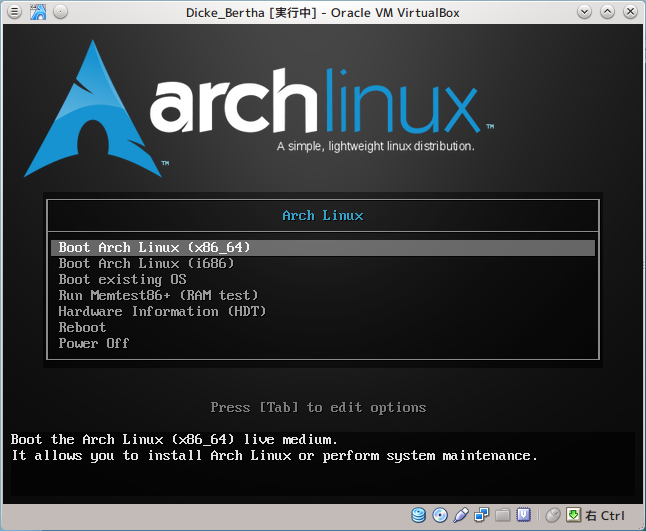
\includegraphics[scale=0.5]{Figs/Fig_ArchLinux/syslinux}\protect\caption{起動するOSを選択する(ブートローダ)}
\label{Choose_OS_syslinux}
\par\end{centering}

\end{figure}


OSを選択後、しばらくすると図\ref{StartPoint}のような画面が表示されます。これがArch Linuxです。

以降では、このようにキーボードでコマンドを逐次叩いていくCUIによって、OSをインストールしていきます。

\begin{figure}[!tbh]


\begin{centering}
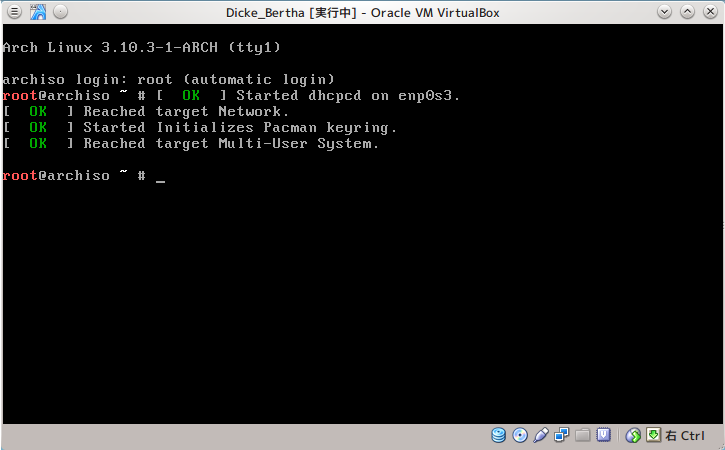
\includegraphics[scale=0.5]{Figs/Fig_ArchLinux/booted}\protect\caption{Arch Linuxの起動}
\label{StartPoint}
\par\end{centering}

\end{figure}



\section{Arch Linuxをインストールする}

それでは早速インストールを始めていきましょう。

インストールの基本的な流れは以下の通りです。
\begin{enumerate}
\item インストールイメージを起動する
\item キーマップを変更する
\item ネットワークへの接続を確認する
\item ディスクを必要な領域ごとに切り分ける(パーティションを作成する)
\item 4.で作成したパーティションにファイルシステムを作成する
\item 5.で作成したファイルシステムをマウントし、OSのプログラムをディスクへ流し込む
\item ディスク上のOSの設定を行う
\item rootアカウントのパスワードを設定する
\item ブートローダをインストールする
\item システムを再起動させてディスクから起動し、rootアカウントでログイン、動作を確認する
\end{enumerate}
現在までに1.が終了しました。以下では順を追って作業を進めていきます。

ここで、本文中ではコマンドを扱いますが、コマンド名は本文中ではタイプライタ体(\texttt{typewriter type})で表現し、実際にコマンドを用いての作業内容はタイプライタ体文字列を影付き枠で囲うことで表します。必要があれば、コマンド実行中の画面あるいは画面の一部を二重枠で囲うことで表します。ここでコマンドを記述する行の先頭に``\texttt{\$}''や``\texttt{\#}''が書かれる場合がありますが、これは実際の作業画面に於けるプロンプトを再現したものであり、実際には入力の必要はありません。加えて、斜体(\texttt{\textit{Italic}})で表現されている箇所は字体に関わらず各位による変更を必要とする箇所を示します。また本文中では、「コマンドを入力する」という行為を簡略のため「叩く」と表現します。

本文中で扱われるコマンドについては適宜必要と思われる部分に関する説明を加えていきますが、いまいちピンとこない場合などは、manを用いることでコマンドの詳細な説明を得ることができます。

\begin{center}
\shadowbox{\begin{minipage}[t]{0.6\textwidth}%
\texttt{\$ man }\texttt{\textit{command\_name}}%
\end{minipage}}
\par\end{center}

と叩くと\texttt{command\_name}という名前のコマンドに関する説明を閲覧できます。


\subsection{キーマップを変更する}

Arch Linuxのデフォルトのキー配列はUS仕様になっています。ですが日本語を第一言語とする方々の大多数はJIS配列のキーボードを使用しているはずです%
\footnote{US配列のキーボードを使用している方はこの小節は読み飛ばして構わない。%
}。このため、キー配列を変更しないと、例えばダブルクォーテーション(``)を入力したいのにアットマーク(@)が入力されたり、括弧を閉じたいのに閉じなかったりと非常にイライラするので、キー配列をJIS配列に変更します。

\begin{center}
\shadowbox{\begin{minipage}[t]{0.6\textwidth}%
\texttt{\# loadkeys jp106}%
\end{minipage}}
\par\end{center}

と叩き、キー配列を変更しましょう。


\subsection{ネットワークへの接続を確認する}

Arch LinuxのインストールイメージにはインストールするOSのプログラムは実は入っていません。インストールイメージはOSという家を建てるための足場のようなものです。OSのプログラムは、Arch
Linuxのサーバから持ってこなければなりません。よって、インターネットへの接続が確立しているか確かめる必要があります。

固定IPアドレスを割り当ててインターネットへ接続している等、特に特殊な環境でない限り、Arch Linuxのインストールイメージは\texttt{dhcpcd}というネットワークデーモン%
\footnote{デーモンとは、システム上で動いているプロセスのうち、表に出てこない(バックグラウンドで実行されている)ものを指す。%
}により、既にインターネットへ接続されています。ここでは接続が確立していることを確かめるにとどめます。

\begin{center}
\shadowbox{\begin{minipage}[t]{0.6\textwidth}%
\texttt{\# ping -c 3 www.tmu.ac.jp}%
\end{minipage}}
\par\end{center}

と叩き、接続を確認します。\texttt{ping}とは引数に指定したサーバへ少量のネットワークパケットを送信してサーバとの通信状態を確認するコマンドです。今回はオプションに``\texttt{-c
3}''を加えて、パケットの転送回数を3回に制限しました。


\subsection{ディスクを必要な領域ごとに切り分ける(パーティションを作成する)}


\subsubsection{ディスクの確認}

続いて、ディスク上にパーティションを作成していきます。パーティションとはディスクの記憶領域が分割されたものです。例えば10GBのディスクを2GBと8GBに分割したとすれば、そのディスクは2GBのパーティションと8GBのパーティションを持つことになります。

パーティションの作成はこだわり出すと止まらなくなることがままあるので、ここはベターな作成法として、ディスクを分割せずに、ディスクをまるごと1つのパーティションとして扱うことにします。

通常仮想マシンのディスクはインストールイメージには``/dev/sda''として認識されています。後述しますが、``/dev''とはコンピュータに接続されたデバイス(\uline{dev}ice)を管理するディレクトリ%
\footnote{別称フォルダ。今後はいわゆるフォルダもディレクトリと呼称する。%
}で、sdaとはシステムに最初に認識されたディスクであるという意味です。今扱っている仮想マシンではディスクは1個のみですので、システムでは``/dev/sda''と認識されています。確認したい場合は、

\begin{center}
\shadowbox{\begin{minipage}[t]{0.6\columnwidth}%
\texttt{\# lsblk}%
\end{minipage}}
\par\end{center}

と叩き、sdX(Xはa--zの間の任意の一字。通常はa)の行を探しましょう。通常は先頭に表示されているはずです。発見したら、その行の``SIZE''の列を確認し、インストール先のディスクの容量と一致しているかを確かめると良いでしょう。


\subsubsection{パーティションの作成}

いよいよパーティションを作成します。以下では、ディスクが``/dev/sda''と認識されていることを仮定します。

ディスクにおけるパーティションの情報は、パーティションテーブルとよばれるもので管理されています。現在、このパーティションテーブルの方式にはMBR(master
boot record)とGPT(GUID partition table)との2種類があります\cite{AP}。MBRは枯れた方式で、GPTはモダンな方式です。ここでは新しさを求めてGPTでのパーティション管理を試みます。

まず以下を叩きます。\texttt{cgdisk}とは、ディスク上にGPTパーティションを作成するためのユーティリティです。

\begin{center}
\shadowbox{\begin{minipage}[t]{0.6\textwidth}%
\texttt{\# cgdisk /dev/sda}%
\end{minipage}}
\par\end{center}

すると図\ref{cgdisk}のような表示になるはずです。まれに``Warning! Non-GPT or damaged disk
detected!''などと怒られる場合がありますが、どうせ新たにパーティションを作るのですからシカトしてEnterを押下しましょう。

\begin{figure}[!tbh]


\begin{centering}
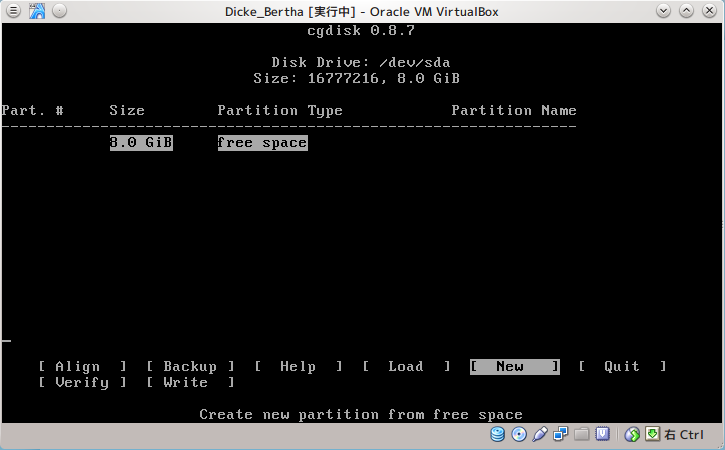
\includegraphics[scale=0.5]{Figs/Fig_ArchLinux/cgdisk}\protect\caption{cgdisk}
\label{cgdisk}
\par\end{centering}

\end{figure}


まず``New''を選択(左右矢印キーで選択可)するかNキーを押下してパーティションの作成に入ります。あとは元の表示になるまでずっとEnterキーを叩けば良いのですが、折角ですので尋ねられる文章の意味を記しておきます。
\begin{itemize}
\item First Sector (XXXX--YYYY, default=XXXX)(XXXX、YYYYは適当な値)

\begin{itemize}
\item パーティションの開始位置を指定する。XXXXはディスク先頭0バイトからXXXXバイト目を示す。
\end{itemize}
\item Size in Sectors or \{KMGTP\} (default=XXXX)(XXXX、YYYYは適当な値)

\begin{itemize}
\item パーティションのサイズを指定する。デフォルト値XXXXは今作成しているパーティションの後ろに別のパーティションが存在しないため、ディスクのサイズに等しくなっている。\\
セクタ(Sector)というのは容量の単位。KMGTPも同様(KiB、MiB、GiB、TiB、PiB)%
\footnote{2バイト接頭辞。それぞれ$\mathrm{2^{10}B}$、$\mathrm{2^{20}B}$、$\mathrm{2^{30}B}$、$\mathrm{2^{40}B}$、$\mathrm{2^{50}B}$を意味する。%
}
\end{itemize}
\item Current type is 8300(Linux filesystem)\\
Hex code or GUID (L to show codes, Enter = 8300)

\begin{itemize}
\item パーティションのタイプを指定している。Linux用パーティションの場合8300が該当する。
\end{itemize}
\item Current partition name is ''\\
Enter new partition name, or \textless{}Enter\textgreater{} to use
the current name:

\begin{itemize}
\item パーティション名を決める。デフォルトでは名無しのパーティションとなる。
\end{itemize}
\end{itemize}
\begin{figure}[!tbh]
\begin{centering}
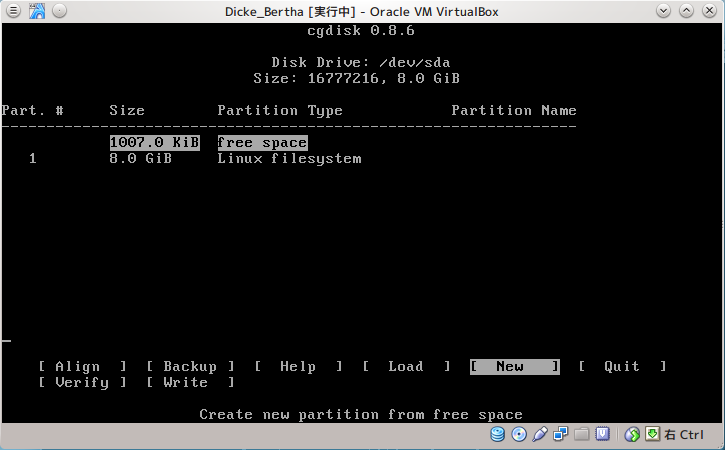
\includegraphics[scale=0.5]{Figs/Fig_ArchLinux/cgdisk_created}\protect\caption{cgdisk(パーティション作成後)}
\label{cgfisk_created}
\par\end{centering}

\end{figure}


もとの表示(図\ref{cgfisk_created})に戻ったら、まず作成したパーティションを上下矢印キーを用いて選択し、次に左右矢印キーを用いて``Write''を選択するかShiftキーを押しながらWキーを押して%
\footnote{以後このようなキー操作を``Shift+W''のように表現する。%
}パーティションをディスクへ書き込む作業へ入ります。``Areyou sure you want to write the partition
table to disk? (yes or no):''と聞かれるので、yesと入力し(``y''でないことに注意)パーティションをディスクに書き込みます。書き込みが終了したら再び図\ref{cgfisk_created}の表示に戻るので、左右矢印キーを用いて``Quit''を選択するかQキーを押してcgdiskを終了します。

パーティションの作成の確認には\texttt{lsblk}を使用すると良いでしょう。

\begin{center}
\shadowbox{\begin{minipage}[t]{0.6\textwidth}%
\texttt{\# lsblk}%
\end{minipage}}
\par\end{center}

を叩き、``sda''を確認すると、その直下に``sda1''が新たに表示されているはずです。この行の``TYPE''を確認すると、``PART''となっていると思います。これはPARTitionの意で、sdX1はディスクsdXに作成されたパーティションを意味しています。ちなみに、sdaにパーティションを何個も作っていくと、もちろんsda2、sda3、$\ldots$と認識されていきます。


\subsection{ファイルシステムの作成}

以上までの作業で、OSという家を建てる上での地均しは終了しました。次に基礎を築きます。

今回はパーティションをext4(Fourth Extended File System)というファイルシステムでフォーマットします。ファイルシステムとは、ディスク上に存在するファイルを管理するためのシステムで、OSの機能の一部です。

/dev/sda1をext4でフォーマットするには、以下を叩きます%
\footnote{\cite{ALBG}では\texttt{mkfs.ext4 /dev/sda1}となっているが、この文書でのコマンドの用法の統一のため異なる形式を用いた。%
}。

\begin{center}
\shadowbox{\begin{minipage}[t]{0.6\textwidth}%
\texttt{\# mkfs -t ext4 /dev/sda1}%
\end{minipage}}
\par\end{center}

以後の説明では、適宜「ディスク」と「ファイルシステム」を同義なものとして扱います。ハードウェアとしてのディスクを扱う場合、文脈上に説明を加えることとします。


\subsection{ファイルシステムのマウント}


\subsubsection{ファイルとディレクトリ階層}

マウントとは、コンピュータに接続されたデバイスを、OSが管理および制御できる状態にすることを指します。ファイルシステムをマウントする場合、Linuxを始めとするUnix互換OSでは\texttt{mount}というコマンドを用います。

元来、Linuxには``すべてのものはファイルである(everything-is-a-file)''という思想があります\cite{LSP}。つまり、ディスクやCDドライブ、ディスプレイやプリンタやキーボード、はたまたディレクトリや通常の意味でのファイル、さらにプロセスに至るまでの全てがLinuxにおいてはファイルとして扱われます。アクセスの方法も道具の相異は有りますがほぼ統一されており、それは単純に読み書きとして表現できます。

さて、Linuxのファイルは``/''で表現されるルートディレクトリを頂上に、全てのファイルとディレクトリは``/''の下に位置します。厳密にはファイルの目的に応じて、``/''直下にいくつかのディレクトリが存在し、ファイルとディレクトリは``/''直下のディレクトリに振り分けられて存在しています。Linuxのとるこのようなディレクトリ階層はFHS(Fileystem
Hierarchy Standaed)と呼ばれ、標準化されていますが、実際のLinuxディストリビューション同士では細かい差異が存在しています。

Arch Linuxにおけるディレクトリ階層は図\ref{AFH}のようになります\cite{FHS}\cite{AFH}。

\begin{figure}[!tbh]


\centering{}%
\fbox{\begin{minipage}[t]{1\columnwidth}%
\begin{tabbing}
1234567890123456\=7890\=12345678901234567890 \kill
/			   \>rootディレクトリ(システムの最上位ディレクトリ)\\
├bin  	 	\>全てのユーザ用の基本コマンドを格納するディレクトリ \\
│	 	 	\>\>(現在は/usr/binへのシンボリックリンク)\\
├boot 	 	\>ブートローダ用ファイルとカーネルイメージを格納するディレクトリ \\
├dev  	 	\>デバイスファイルを格納するディレクトリ \\
├etc  	 	\>OSの設定ファイルを格納するディレクトリ \\
├home 	 	\>一般ユーザ用ディレクトリ \\
├lib  	 	\>共有ライブラリとカーネルモジュールを格納するディレクトリ \\
│	 	 	\>\>(現在は/usr/libへのシンボリックリンク)\\
├(lib64)   	\>64bit環境用の共有ライブラリを格納するディレクトリ\\
│			  \>\>(現在は/usr/libへのシンボリックリンク)\\
├lost+found	\>ファイルシステム障害発生時に復旧可能なファイルの一時保管場所 \\
├mnt 		  \>ファイルシステムの一時的なマウントポイントを格納するディレクトリ \\
├opt 		  \>通常のLinuxのディレクトリ階層では扱えないプログラムを格納するディレクトリ \\
├proc 		 \>カーネル及びプロセスの情報を格納するディレクトリ \\
├root 		 \>rootユーザ用ディレクトリ \\
├run 		  \>短期的に使用されるファイルを格納するディレクトリ \\
├sbin 		 \>システム管理用コマンド等を格納するディレクトリ \\
│			  \>\>(現在は/usr/binへのシンボリックリンク) \\
├srv 		  \>HTTP、FTP等のサービス用のデータ \\
├sys 		  \>OS全体の情報を格納するディレクトリ \\
├tmp 		  \>一時的なファイルを格納するディレクトリ \\
├usr 		  \>各種プログラム等を格納するディレクトリ \\
└var 		  \>頻繁に変更されるデータを格納するディレクトリ
\end{tabbing}%
\end{minipage}}\protect\caption{Arch Linuxのディレクトリ階層}
\label{AFH}
\end{figure}



\subsubsection{ファイルシステムのマウント}

\cite{ALBG}によれば、OSをインストールするディスクを/mnt下にマウントしています。この文書に於いても\cite{ALBG}に従い、/mnt下にマウントすることにしましょう。また、今回はディスク上にはファイルシステムが1つしか存在しませんので、そのファイルシステムを``/''として扱い(以下``/ファイルシステム''と呼称します。)/mntにマウントします。ちなみに、ファイルシステムは通常データを階層的に管理するために扱われるため、ファイルシステムをマウントするときはディレクトリにマウントしないとエラーが起きます。

\begin{center}
\shadowbox{\begin{minipage}[t]{0.6\textwidth}%
\texttt{\# mount /dev/sda1 /mnt}%
\end{minipage}}
\par\end{center}

と叩き、ファイルシステムをマウントします。注意すべきことして、マウントするのはディスクではなくファイルシステムですので、\texttt{mount}に指定する引数は/dev/sdaではなく/dev/sda1です。


\subsection{OSをインストールする}

いよいよOSをインストールします。

OSをインストールする前に、まずはOSのインストールに必要なパッケージをダウンロードするサーバを決めます。

OSを構成するパッケージは、必要なものを全てひっくるめると数百MBもの大きさになり、パッケージ群を提供するサーバ及び通信回線に多大な負荷を及ぼします。更に、このパッケージ群を必要とするクライアントは何百何千、何万何十万という数になりますから、これを1台のサーバで賄おうとした場合サーバは通常処理能力の限界を瞬時に迎え即死します。このため、通常大規模なデータを多数のクライアントから要求されるような状況で扱う場合は、負荷分散のためミラーサーバと呼ばれるサーバを複数台用意し、特定のサーバに負荷が集中しないようにしています。

サーバを分散することで得するのは運営側のみではありません。同じデータをダウンロードするにしても、例えば日本にいる利用者が日本にあるサーバからダウンロードするのとブラジルにあるサーバからダウンロードするのとでは掛かる時間は雲泥の差です。回線の性能や使用状況等による差異も有りますが、同程度の回線を使用しているならば、物理的な距離の近い経路からアクセスしたほうが、一般にダウンロードに要する時間は少なく済むであろうことは直感的にも納得できると思います。

Arch Linuxは現在世界各国にミラーサーバを構え、日本国内にも北陸先端科学技術大学院大学(通称JAIST)が提供するものと、筑波大学が提供するものとの2種類があります。察しがつくと思いますが、インストールイメージを入手する際に説明した2つのサーバである\texttt{jaist.ac.jp}と\texttt{ftp.tsukuba.wide.ad.jp}がそれぞれ該当します。どのミラーサーバにアクセスするかを設定するには/etc/pacman.d/mirrorlistを編集します。どちらのサーバを選んでも良いのですが、今回はJAISTのサーバを使う方法でいきたいと思います。筑波大学のサーバを使う場合も、以後で解説する方法と同様に行うことが可能です。


\subsubsection{ミラーサーバの設定}

/etc/pacman.d/mirrorlistを設定します。

このファイルは前述の通り、パッケージのダウンロードにどのサーバを使うかを指定するための設定ファイルです。Linuxの設定ファイルはほぼ全てテキストファイルですので、設定を変更したりする場合にはテキストエディタを使用します。今回は一般的なテキストエディタに近い使用感を持つ\texttt{nano}というエディタを使用します。以後の設定ファイルの編集に於いても\texttt{nano}を使用していきます。

\begin{center}
\shadowbox{\begin{minipage}[t]{0.6\textwidth}%
\texttt{\# nano /etc/pacman.d/mirrorlist}%
\end{minipage}}
\par\end{center}

と叩くと、図\ref{mirrorlist_nano}のような表示になります。これが\texttt{nano}のインターフェースです。

\begin{figure}[!tbh]


\begin{centering}
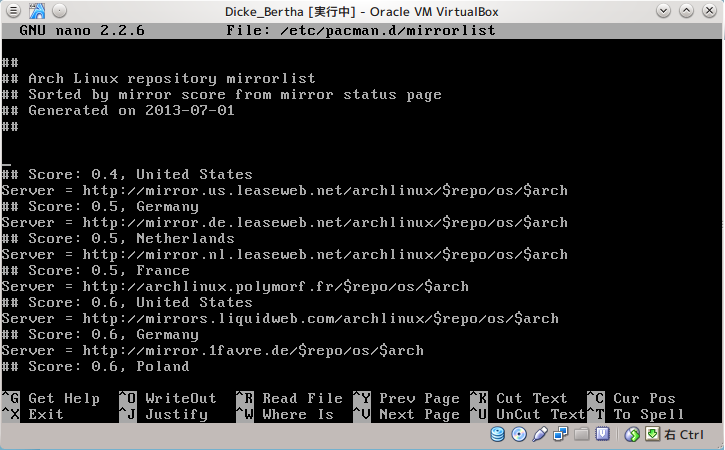
\includegraphics[scale=0.5]{Figs/Fig_ArchLinux/mirrorlist_nano}\protect\caption{nanoによる/etc/pacman.d/mirrorlistの編集}
\label{mirrorlist_nano}
\par\end{centering}

\end{figure}


このファイルには世界に点在するArch LinuxのミラーサーバのURLが収録されています。このまま何も変更も加えずにパッケージのダウンロードを試みると、有効なサーバとして\texttt{mirror.us.leaseweb.net}が選択、使用されます。これはアメリカに存在するサーバです。行頭に``\#''がついている行はコメントアウトされた行といい、データとして意味を成さない記述となります。文字通り「コメント」を書き込む際に用いられるものです。従って、コメントアウトされていない行のうち最も上位にある\texttt{mirror.us.leaseweb.net}が選択されます。

即ち、\texttt{mirror.us.leaseweb.net}よりも上にJAISTのサーバのURLを書き込めば、パッケージのダウンロードはJAISTのサーバより行われることとなります。では早速JAISTのサーバのURLを探し出しましょう。

まずCtrl+Wを入力してファイル内の文字列検索へ移行します。

\begin{center}
\doublebox{\begin{minipage}[t]{0.6\textwidth}%
\texttt{Search:}%
\end{minipage}}
\par\end{center}

という表示が画面下部に現れますので、そこへ``japan''と入力し、Enterキーを押下します。するとファイル内で``Japan''の文字列が含まれる行へカーソルが移動します。該当するものが複数個存在する場合、現在のカーソル位置から最も近い行へ移動します。/etc/pacman.d/mirrorlistではJAISTのサーバと筑波大学のサーバと両方が含まれていますが、JAISTのサーバのほうがファイル内で上位に記載されているので、通常はJAISTのサーバのURL付近にカーソルが移動するはずです。

続いてJAISTサーバのURLへ上下矢印キーでカーソルを合わせたら、Alt+6でカーソルの存在する行全体をコピーします。次にPgUpキーでファイルの上方へ移動し、\texttt{mirror.us.leaseweb.net}よりも上の行にコピーしたURLを貼り付けます。コピーした内容の貼付けにはCtrl+Uとします。

\begin{figure}[!tbh]


\begin{centering}
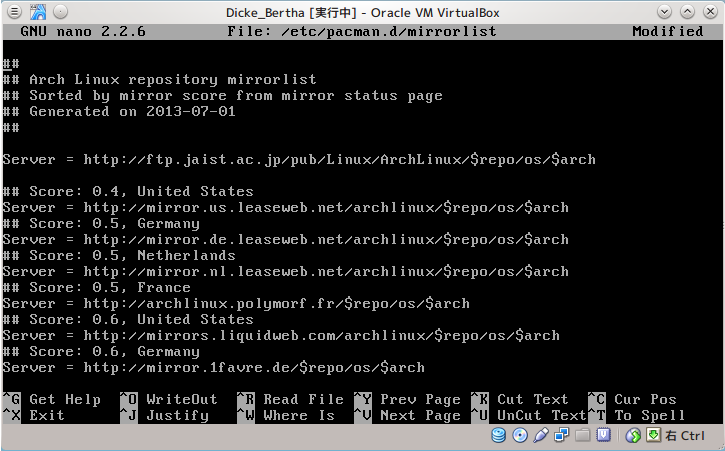
\includegraphics[scale=0.5]{Figs/Fig_ArchLinux/mirrorlist_nano_modified}\protect\caption{編集後の/etc/pacman.d/mirrorlist}
\label{mirrorlist_nano_modified}
\par\end{centering}

\end{figure}


図\ref{mirrorlist_nano_modified}のように編集が完了したら、ファイルを保存しエディタを閉じます。まずCtrl+Oを入力し、ファイルを保存します。このとき、

\begin{center}
\doublebox{\begin{minipage}[t]{0.6\textwidth}%
\texttt{File Nameto Write: /etc/pacman.d/mirrorlist}%
\end{minipage}}
\par\end{center}

と表示されます。コロン以降を変更すればファイル名の変更が可能ですが、今回はそのままEnterを押下します。すると

\begin{center}
\doublebox{\begin{minipage}[t]{0.6\textwidth}%
\texttt{Wrote XXX lines}%
\end{minipage}}
\par\end{center}

と表示され、ファイルが保存されます(XXXはファイルの行数を示す整数)。続いて、Ctrl+Xを入力し、\texttt{nano}を終了します。


\subsubsection{パッケージのダウンロード}

いよいよ正真正銘のOSのインストールです。

OSインストールにはpacstrapというスクリプトを使用します。これは後述するpacmanのラッパ%
\footnote{ある関数を使うために、関数および関数に必要なデータや引数、別の関数などを一緒にまとめて定義した関数。ここでは「関数」を「コマンド」に置き換えたものが該当する。wrapper。%
}であり、このスクリプトを使うことで、OSのインストール先を指定してやるだけでほぼ何も考えずにOSのインストールが自動で成されるというスグレモノなのです。

\begin{center}
\shadowbox{\begin{minipage}[t]{0.6\textwidth}%
\texttt{\# pacstrap -i /mnt base}%
\end{minipage}}
\par\end{center}

と叩き、インストールを開始します。コマンドの意味は、/mntにbaseカテゴリのパッケージのみをインストールする、というものです。baseカテゴリにはこれさえあれば最低限は使えるというパッケージが含まれています%
\footnote{私達が通常想起する「最低限」とは程遠いことに注意。もっと低い次元の「最低限」である。%
}。


\subsubsection{/etc/fstabの編集}

OSのインストールも折り返し地点に近づいてきました。続いて/etc/fstabの編集に移ります。

OS起動後、OSはシステムが格納されているファイルシステムをマウントしなければなりません。(詳しくはファイルシステム内にOSが存在するため、OS起動前にファイルシステムは認識できません。このあたりの詳細は後述します)OS起動後にOSがマウントすべきファイルシステムを記載した設定ファイルが/etc/fstabです。これが正しく設定されていないとOSは起動時にエラーを出力し、起動に失敗します。

/etc/fstabを編集する前に、まずは/etc/fstabを作成しましょう。以下を叩きます。

\begin{center}
\shadowbox{\begin{minipage}[t]{0.6\textwidth}%
\texttt{\# genfstab -L -p /mnt \textgreater{}\textgreater{} /mnt/etc/fstab}%
\end{minipage}}
\par\end{center}

\texttt{genfstab}で/mntにマウントされているファイルシステムにおけるfstabを作成し、それを/mntにマウントされているファイルシステムに書き込みます。

続いて/etc/fstabを編集していきます。

\begin{center}
\shadowbox{\begin{minipage}[t]{0.6\textwidth}%
\texttt{\# nano /mnt/etc/fstab}%
\end{minipage}}
\par\end{center}

と叩くと、以下のような表示がなされると思います。

\begin{center}
\doublebox{\begin{minipage}[t]{0.9\textwidth}%
{\tt
\begin{tabbing}
123456789012345\=6789012\=345678901\=234567890123456789012345678\=9012345\=67890 \kill
\# \\
\# /etc/fstab: static file system information \\
\# \\
\#<file system> \><dir>  \><type>   \><options>                  \><dump> \><pass> \\
\# /dev/sda1 UUID=d9a74548-5c57-23c6-91f2-888a1bc2fd67 \\
/dev/sda1      \> /      \> ext4   \> rw,relatime,data=ordered  \> 0      \> 1
\end{tabbing}
}%
\end{minipage}}
\par\end{center}

チェックすべきは一箇所で、``\texttt{\textless{}pass\textgreater{}}''の列の値が``1''となっているかを確認してください。他は特にいじらなくて良いと思います。


\subsection{OSの設定を行う}

OSのインストール自体は完了しました。以後はOSの設定やユーザの追加、各種パッケージの追加、ブートローダのインストールを行います。


\subsubsection{chroot(arch-chroot)}

現在使用しているArch LinuxというOSは言うまでもなくインストールメディアとしてのArch Linuxであり、ディスクにインストールしたArch
Linuxではありません。ディスク上にインストールされたOSの設定を行うには、やはりOSをインストールしたディスク内の設定ファイルを変更しなければなりません。ですが、今の状態ではファイルシステムが/mntにマウントされている都合上、設定ファイルのパスの先頭に``/mnt''を付けなくてはならず、面倒です。加えて、ディスク上のOSでコマンドを実行したい場合も、同じくマウントしたファイルシステム経由ではいささか不都合が生じます。

というわけで、ディスク上のOSを操作できるようにしましょう。これには、\texttt{chroot}のラッパである\texttt{arch-chroot}というスクリプトを用います。これはrootファイルシステムを変更(\uline{ch}ange
\uline{root} filesystem)するためのものです。

\begin{center}
\shadowbox{\begin{minipage}[t]{0.6\textwidth}%
\texttt{\# arch-chroot /mnt}%
\end{minipage}}
\par\end{center}

と叩くことで、/mntにマウントされたファイルシステムをrootファイルシステムとして扱います。これはディスク上にインストールされたOSを起動している状態と同等です。


\subsubsection{キーマップの変更}

環境が変更されたのでキー配列もデフォルトのUS仕様になっています。

\begin{center}
\shadowbox{\begin{minipage}[t]{0.6\textwidth}%
\texttt{\# loadkeys jp106}%
\end{minipage}}
\par\end{center}

と叩き、キー配列を変更しましょう。

また、これは一時的な変更であり、インストール完了後システムを再起動すると設定は無効化され、キー配列は再びUS配列に戻ってしまいます。これを阻止するには、/etc/vconsole.confに所定の設定を記述する必要があります。

\begin{center}
\shadowbox{\begin{minipage}[t]{0.6\textwidth}%
\texttt{\# nano /etc/vconsole.conf}%
\end{minipage}}
\par\end{center}

を実行してファイルを開き、そこへ

\begin{center}
\doublebox{\begin{minipage}[t]{0.6\textwidth}%
\texttt{KEYMAP='jp106'}%
\end{minipage}}
\par\end{center}

と記述します。

なお、これはコンソール上、即ちCUI上のみで有効な設定です。GUIに於いては設定が反映されない場合があります。GUI上におけるキーマップの設定は、第\ref{chap:Arch-Linux=003092=004F7F=007528=003059=00308B}章で扱います。




\subsubsection{ロケールの設定}

ロケール(Locale)とは、ユーザが扱う言語を規定するものです。この分野の標準語は事実上英語であり、デフォルトではArch Linuxも英語が使用されていますが、ロケールを変更することにより、英語以外の言語を使用することができます。用意されている言語はヨーロッパ方面に限らず全世界にまたがっています。

ですが、ここでは扱う言語は英語のままとします。というのも、ASCIIに含まれない文字コードを扱う場合、特に何も設定していないCUI上では文字化けを起こすためです。残念ながら我々の日本語はASCIIには含まれない文字コードを扱うので、使えません。では日本語は使えないのかというとそういうわけではなく、CUIでは英語、GUIでは日本語というように設定することが可能です。詳細は第\ref{chap:Arch-Linux=003092=004F7F=007528=003059=00308B}章で扱います。

ではロケールの設定をしましょう。最初に、使用するロケールを設定します。これは/etc/locale.genによって設定されています。これを編集します。以下のように叩きます。

\begin{center}
\shadowbox{\begin{minipage}[t]{0.6\textwidth}%
\texttt{\# nano /etc/locale.gen}%
\end{minipage}}
\par\end{center}

ロケール名は、``xx\_yy.ZZZ''というフォーマットになっています。xxは言語コード、yyは国名コード、ZZZは文字コードをそれぞれ示します。例えばロケール名が``en\_US.UTF-8''である場合、このロケールは文字コードにUTF-8を用いるアメリカ英語であるという意味になります。

先程「CUIでは英語、GUIでは日本語というように設定することが可能」と説明しましたが、/etc/locale.genが扱う内容はシステムすべてのロケールであり、ここで日本語を扱うように設定しないと、システム上で日本語を扱うことが不可能になります。ちなみにロケールは複数選択が可能です。

ここでは以下のロケールをアンコメント%
\footnote{コメント行の先頭にある``\#''を削除すること。これにより記述が設定として反映される。%
}します。
\begin{itemize}
\item en\_US.UTF-8
\item en\_US.ISO-8859-1
\item ja\_JP.EUC-JP
\item ja\_JP.UTF-8
\end{itemize}
設定ファイルを編集したら、今度は設定を反映させます。

\begin{center}
\shadowbox{\begin{minipage}[t]{0.6\textwidth}%
\texttt{\# locale-gen}%
\end{minipage}}
\par\end{center}

と叩くことで設定が反映されます。

続いて、CUI上で使用する言語を規定します。これは/etc/locale.confで設定されます。今回は英語を使用するので、/etc/locale.confには

\begin{center}
\doublebox{\begin{minipage}[t]{0.6\textwidth}%
\texttt{LANG=''en\_US.UTF-8''}%
\end{minipage}}
\par\end{center}

とだけ書いて保存します。


\subsubsection{タイムゾーンの変更}

続いてシステムの時間を設定します。インターネットに接続していれば、時刻サーバと標準時が自動的に同期されるため、正しいタイムゾーンを設定すれば時刻は自動的に正しい時刻に補正されます。

Linuxでは日本標準時はおおよその場合``Asia/Tokyo''として表現されます。タイムゾーンの情報は/usr/share/zoneinfo/下に置かれています。日本のタイムゾーンの情報は、/usr/share/zoneinfo/Asia/Tokyoとなります。これを/etc下に置きますが、ファイルのコピーを置くのではなく/usr/share/zoneinfo/Asia/Tokyoへのシンボリックリンク%
\footnote{あるファイルへのアクセスを異なる場所から行うための手段。ここでは/usr/share/zoneinfo/Asia/Tokyoへのアクセスにそれを直接指定するのではなく/etc/localtimeを指定することで/usr/share/zoneinfo/Asia/Tokyoへアクセスが可能となる。%
}を/etcに置くようにします。シンボリックリンクの名称は/etc/localtimeとします。

\begin{center}
\shadowbox{\begin{minipage}[t]{0.6\textwidth}%
\texttt{\# ln -s /usr/share/zoneinfo/Asia/Tokyo /etc/localtime}%
\end{minipage}}
\par\end{center}


\subsubsection{ハードウェア時刻の変更}

次にハードウェアの時刻を設定します。適切なハードウェア時刻を設定しないと、システムの時刻に誤差が生じる可能性があります。

\cite{ALBG}によれば、ハードウェア時刻にはUTC%
\footnote{協定世界時(coordinated universal time)。標準時の基準となるもの。%
}を設定することが推奨されているので、以下のように叩きます。

\begin{center}
\shadowbox{\begin{minipage}[t]{0.6\textwidth}%
\texttt{\# hwclock -{}-systohc -{}-utc}%
\end{minipage}}
\par\end{center}


\subsubsection{ホスト名の変更}

ホスト名とはいわばコンピュータの名前です。ネットワーク上でコンピュータを指し示すものとして扱われます。

設定自体は/etc/hostnameというファイルに記載された文字列がホスト名として認識されますが、今回は引数をそのまま標準出力%
\footnote{通常はディスプレイを意味する。%
}に表示する\texttt{echo}というコマンドと、得られた出力を入力として別の処理へ与えるリダイレクトという機能を用いて簡潔に設定することにします。

\begin{center}
\shadowbox{\begin{minipage}[t]{0.6\textwidth}%
\texttt{\# echo ``}\texttt{\textit{HOSTNAME}}\texttt{'' \textgreater{}
/etc/hostname}%
\end{minipage}}
\par\end{center}

と叩くことで、ホスト名が\textit{HOSTNAME}に設定されます。詳細を説明すると、まずechoによって\textit{HOSTNAME}は標準出力に出力されますが、リダイレクトが使用されているので、\textit{HOSTNAME}はそのままリダイレクト先への入力として扱われます。リダイレクトは入力文字列としてHOSTNAMEを受け取り、そのまま出力先に指定された/etc/hostnameに内容を書き込みます。

処理結果を確認するには、エディタを用いるか、\texttt{cat}というコマンドを用いて

\begin{center}
\shadowbox{\begin{minipage}[t]{0.6\textwidth}%
\texttt{\# cat /etc/hostname}%
\end{minipage}}
\par\end{center}

とすれば良いでしょう。\texttt{cat}は引数に指定したファイルを標準出力上に表示するコマンドです。


\subsubsection{ネットワークの設定}

Arch Linuxでは、ネットワーク管理の為のネットワークマネージャとして、規定としてはnetctlを使用します\cite{An}。netctlはCUIベースのネットワークマネージャであり、GUIを用いたネットワークマネージャのような直感的な使い勝手はありませんが、テキストファイルから構成される簡潔な設定ファイルを用いることで柔軟なネットワーク設定を行うことが出来ます。

netctlはchrootされた環境では動作出来ません。ここでは、以下を叩くことでnetctlを動作させる為の依存関係を解決するにとどめておきましょう。netctlについては第\ref{chap:Arch-Linux=003092=004F7F=007528=003059=00308B}章で扱います。

\begin{center}
\shadowbox{\begin{minipage}[t]{0.6\textwidth}%
\texttt{\# pacman -S dhclient}%
\end{minipage}}
\par\end{center}

ネットワークへの接続にイーサネットによる有線接続でなくwifiによる無線接続を用いる場合は、こちらも依存関係を満たすためにwpa\_supplicantというパッケージをインストールする必要があります。当該環境においては、上記の代わりに下記を叩いてください。

\begin{center}
\shadowbox{\begin{minipage}[t]{0.6\textwidth}%
\texttt{\# pacman -S dhclient wpa\_supplicant}%
\end{minipage}}
\par\end{center}


\subsection{rootアカウントのパスワードを決定する}

OSを使用するユーザのアカウントには通常一般ユーザとスーパーユーザの2種類が存在します%
\footnote{厳密にはこの2種類に加え、特定のプロセスが使用するシステムアカウントと呼ばれる1種類が加わる。%
}。一般ユーザというのは、字面の通り通常用途に使用するユーザのアカウントであり、OS内で行使できる権利に制限があります。例えばシステム全体に影響する設定の変更は一般ユーザには許可されていません。対して、スーパーユーザというのはOS内で行使できる権利に制限のないアカウントです。スーパーユーザの権限は実に強力で、スーパーユーザが定められたOSの中であれば全ての行為が実現できます%
\footnote{実はできないこともある。例えば、如何なるユーザ、グループにも読み書き実行を許可しないファイルへの読み書き実行はスーパーユーザでも不可能。スーパーユーザは全能の存在ではない。%
}。いわばそれはシステムを創造することもでき、またシステムを破壊することもできるのです。ちなみに、スーパーユーザのアカウントはLinuxでは通常rootアカウントと呼ばれています。

デフォルトではrootアカウントのみがシステム上には存在しています。よって、通常は一般ユーザ用のアカウントも新たに作成するのですが、それはインストール作業が完了してから、ということにしましょう。デフォルトのrootアカウントにはパスワードが設定されていません。まずはこちらを先にどうにかしましょう。

\begin{center}
\shadowbox{\begin{minipage}[t]{0.6\textwidth}%
\texttt{\# passwd}%
\end{minipage}}
\par\end{center}

と叩くと、

\begin{center}
\doublebox{\begin{minipage}[t]{0.6\textwidth}%
\texttt{Enter new UNIX password:}%
\end{minipage}}
\par\end{center}

というプロンプトが表示されるので、パスワードを入力します。ここで、キーボードをいくら叩こうとも、入力内容は画面に表示されないことに注意してください。画面に表示されなくとも入力された内容は保持されていますし、ミスタイプした場合はBackspaceキーを使用して訂正することも可能です。

パスワードを入力したら、

\begin{center}
\doublebox{\begin{minipage}[t]{0.6\textwidth}%
\texttt{Retype new UNIX password:}%
\end{minipage}}
\par\end{center}

と表示されますので、再度同じパスワードを入力します。

入力に成功したら、

\begin{center}
\doublebox{\begin{minipage}[t]{0.6\textwidth}%
\texttt{passwd: password updated successfully}%
\end{minipage}}
\par\end{center}

と表示されます。


\subsection{ブートローダをインストールする}

OSは通常ディスク内(詳しくはディスク上のファイルシステム内)に存在するということは既にご存知であると思います。OSがファイルシステムを管理下に置くには、ファイルシステムをマウントしなければなりません。さて、ここで疑問が生じます。ファイルシステム内に存在するOSをコンピュータ起動時に呼び出すにはどうすればいいのでしょう。コンピュータの起動時には当然OSは動作していません。するとOSが起動していないのでハードウェアを制御下に置けません。しかしOSはディスクというハードウェアの中に存在するプログラムです。困ったことになりました。OSを起動するためにはOSが必要ですが、OSを起動するためのOSはどのように起動すればよいのでしょう%
\footnote{似たような問題に「コンパイラをコンパイルするためのコンパイラのコンパイルはどうすればいいのか」というものがあり、これはブートストラップ問題と呼ばれる。「服を買いに行くための服が無い」という問題との類似点が指摘されている[要出典]。ちなみにコンパイラを処理するためのコンパイラのコンパイルは元を辿って行くと最初期には手で行われた(はず)し、そもそもソフトウェアではなかった。%
}。

これを解決するのがブートローダ(ブートストラップローダ)%
\footnote{英語ではbootstrap loaderと書く。ブーツのつまみ革(bootstrap)に由来する。ブーツのつまみ革ってなんだという人は、小学生が履いている上履きのかかと部分についてたアレを思い出すと良いかもしれない。%
}というプログラムで、実はこのブートローダがいわば「OSを起動するためのOS」となるのです。

では早速導入していきましょう。今回はsyslinuxというブートローダを使用します。

\begin{center}
\shadowbox{\begin{minipage}[t]{0.6\textwidth}%
\texttt{\# pacman -S syslinux gptfdisk}%
\end{minipage}}
\par\end{center}

と叩き、syslinuxのパッケージを導入します。続いて、ブートローダの設定のために、

\begin{center}
\shadowbox{\begin{minipage}[t]{0.6\textwidth}%
\texttt{\# syslinux-install\_update -iam}%
\end{minipage}}
\par\end{center}

と叩きます。最後に、syslinuxの設定ファイルである/boot/syslinux/syslinux.cfgを設定します。

デフォルトではカーネルイメージの場所が/dev/sda3となっているのですが、もちろん/dev/sda3というパーティションは存在しないので、これを/dev/sda1に書き換えます。/dev/sda3となっている箇所が複数箇所ある場合は、その都度/dev/sda1に書き換えます。設定を終えたら変更を保存して終了します。


\subsection{インストールの終了}

これでインストールの全工程が終了しました。お疲れ様でした。最後にシステムを終了し、仮想マシンをオフにします。

まずシェル%
\footnote{今までコマンドを入力してきた環境をシェルという。現在使用しているシェルはCUIのシェルであり、GUIのシェルも存在する。%
}上で

\begin{center}
\shadowbox{\begin{minipage}[t]{0.6\textwidth}%
\texttt{\# exit}%
\end{minipage}}
\par\end{center}

と叩くと\texttt{chroot}が終了し、インストールメディアへ帰ってきます。\texttt{exit}は本来ユーザをログアウトするためのコマンドですが、\texttt{chroot}下においては\texttt{chroot}の終了を意味します。

続いて、マウントしていたファイルシステムをアンマウント%
\footnote{字面の通りマウントを解くこと。%
}します。

\begin{center}
\shadowbox{\begin{minipage}[t]{0.6\textwidth}%
\texttt{\# umount /mnt}%
\end{minipage}}
\par\end{center}

と叩くことで、/mntにマウントされていたファイルシステムをアンマウントします。

最後にシステムをシャットダウンしましょう。これには以下のように叩きます。

\begin{center}
\shadowbox{\begin{minipage}[t]{0.6\textwidth}%
\texttt{\# shutdown -h now}%
\end{minipage}}
\par\end{center}

字面の通り、現時点を以って電源を落とせ、という意味です。これによりOSはシャットダウン処理を行い、コンピュータはシャットダウンされます。


\chapter{Arch Linuxを使用する\label{chap:Arch-Linux=003092=004F7F=007528=003059=00308B}}

第\ref{chap:Arch-Linux=00306E=0030A4=0030F3=0030B9=0030C8=0030FC=0030EB}章でArch
Linux自体のインストールは完了しました。しかしOSをインストールしたというだけでは明らかに消化不十分で、実用に耐えうるようなOSを本ゼミの参加者諸氏は必要としているはずです。Arch
Linuxのインストールが完了した直後においては、訓練された人間以外はほぼ何も出来ないと言ってもよい、まっさらな環境が眼前に広がるのみです。しかし、このまっさらな環境は、骨格を既に備え、全ての基本となる、頼もしい環境であるともいえます。

本章ではArch Linuxを一般的な用途に用いる為の諸工程を扱います。まずインターネットに接続するためのネットワークマネージャの設定、Arch
Linuxの標準パッケージマネージャである\texttt{pacman}の紹介と説明、一般ユーザの追加、各種パッケージのインストールとその設定、またシステムそれ自体の各種設定を扱い、最終的に日本語環境下でのブラウジングを可能とする環境を構築します。また補足として、Arch
Linuxを使う上で知っておくと便利と思われるものをいくつか紹介しておくことにします。


\section{netctlの設定}

第\ref{chap:Arch-Linux=00306E=0030A4=0030F3=0030B9=0030C8=0030FC=0030EB}章でも扱った通り、Arch
Linuxは規定のネットワークマネージャとしてnetctlを使用します。netctlはCUIベースのネットワークマネージャで、テキストファイルによる設定ファイルを用いる事で柔軟かつ軽快な動作を可能にしています。またnetctlはArch
Linuxが抱えるプロジェクトの一つでもあり、このためArch Linuxとnetctlの親和性は非常に高いものになっています。

GNU/LinuxをはじめとするUnix系OSには、他にwicd%
\footnote{\url{https://launchpad.net/wicd}%
}やnetworkmanager%
\footnote{\url{https://wiki.gnome.org/Projects/NetworkManager}%
}等のネットワークマネージャがあり、これらはLinuxディストリビューションに依存していない汎用なネットワークマネージャです。もちろんnetctlもまた、Arch
Linuxが抱えるプロジェクトではありますが、汎用のネットワークマネージャです。ここではArch Linuxとの親和性と事前準備に掛かる手間の少なさとから、netctlを使用してネットワークを設定していきます。

netctlは、/etc/netctl下に配置される設定ファイルを元にネットワークを設定します。何も設定されていない状態では、/etc/netctlは以下のような3個のディレクトリが配置されているのみです。ここで``\texttt{hoge/}''はhogeという名前のディレクトリを表現していることとします。

\begin{center}
\shadowbox{\begin{minipage}[t]{0.6\textwidth}%
\texttt{\# cd /etc/netctl \&\& ls}

\texttt{examples/ hooks/ interfaces/}

\texttt{\#}%
\end{minipage}}
\par\end{center}

それでは、設定ファイルを作成しましょう。今回は、現在インターネットをクライアントとして利用する際にはほとんどと言って良い程に広く使われるDHCPを用いた接続を想定しています。本ゼミが扱う範疇には含まれませんが、インターネットを利用する上ではDHCP以外の接続方式も存在します。またIPはIPv4を利用するものとします。

まず、自分の環境でネットワークアダプタがどのような記号で表されるかを確認します。ネットワークアダプタとは、その名の通りネットワークを利用する際に使用するアダプタで、具体的にはイーサネットとかwifiを利用するためにシステムへ組み込む機械の事を指します。これは以下を叩くことで確認が可能です。

\begin{center}
\shadowbox{\begin{minipage}[t]{0.6\textwidth}%
\texttt{\# ip a}%
\end{minipage}}
\par\end{center}

この結果、例えば以下のような結果が得られるでしょう。

\begin{center}
\doublebox{\begin{minipage}[t]{1\textwidth}%
\texttt{1: lo: \textless{}LOOPBACK,UP,LOWER\_UP\textgreater{} mtu
65536 qdisc noqueue state UNKNOWN group default}

\texttt{link/loopback 00:00:00:00:00:00 brd 00:00:00:00:00:00}

\texttt{inet 127.0.0.1/8 scope host lo}

\texttt{valid\_lft forever preferred\_lft forever }

\texttt{inet6 ::1/128 scope host}

\texttt{valid\_lft forever preferred\_lft forever }

\texttt{2: enp0s25: \textless{}BROADCAST,MULTICAST\textgreater{} mtu
1500 qdisc noop state DOWN group default qlen 1000}

\texttt{link/ether 00:26:2d:f5:e6:b0 brd ff:ff:ff:ff:ff:ff }

\texttt{3: wls1: \textless{}BROADCAST,MULTICAST\textgreater{} mtu
1500 qdisc mq state DOWN group default qlen 1000}

\texttt{link/ether 00:26:c6:c6:32:88 brd ff:ff:ff:ff:ff:ff}%
\end{minipage}}
\par\end{center}

最近のインストールであれば%
\footnote{厳密に言えば新しめのudevを使用している場合となる。しかしudevは現在systemdの一部になっている(\url{https://wiki.archlinux.org/index.php/udev})ので、現行のsystemdを用いていればudevも自動的に新しくなる。%
}、この一覧のうち、``enp''で始まる文字列はイーサネットアダプタ(有線LAN)を指し、また``wls''で始まる文字列はwifiアダプタ(無線LAN)を指します。以下では、有線LANを使用する場合と無線LANを使用する場合とのそれぞれについて説明を行います。ただし、以下の説明ではイーサネットアダプタをenp0s25、wifiアダプタをwls1と表すこととします。ちなみに、このようなシステム上でデバイスを指し示す文字列をデバイス名と言います。つまり、この例では、イーサネットアダプタのデバイス名はenp0s25、wifiアダプタのデバイス名はwls1となります。


\subsection{有線LANを使用する場合の設定}

設定ファイルのテンプレートは/etc/netctl/examples/下に格納されています。ディレクトリに格納されているテンプレートは複数あり、多岐に渡る接続方法をサポートしていますが、どのテンプレートがどの接続方式を扱うのかは概ねテンプレートファイルの名前を見れば把握できるようになっています。ここでは有線LAN(イーサネット)でDHCPによりインターネットへ接続するので、以下のように叩きます。

\begin{center}
\shadowbox{\begin{minipage}[t]{0.6\textwidth}%
\texttt{\# cp /etc/netctl/examples/ethernet-dhcp /etc/netctl/}\texttt{\textit{hoge}}%
\end{minipage}}
\par\end{center}

設定ファイルの名前は一目で判別できるような物を選ぶと後で困らなくて済みます。例えば今回のようにイーサネットアダプタがenp0s25と表現されるならば、設定ファイルの名前は``enp0s25-dhcp''とするとよいでしょう。

設定ファイルを作成したら、次に内容を編集します。適当なエディタで設定ファイルを開くと、図\ref{ethernet-dhcp}のような内容になっています。

\begin{center}
\begin{figure}[!tbh]


\begin{centering}
\doublebox{\begin{minipage}[t]{0.6\textwidth}%
\texttt{Description='A basic dhcp ethernet connection'}

\texttt{Interface=eth0}

\texttt{Connection=ethernet}

\texttt{IP=dhcp}

\texttt{\#\# for DHCPv6}

\texttt{\#IP6=dhcp}

\texttt{\#\# for IPv6 autoconfiguration}

\texttt{\#IP6=stateless }%
\end{minipage}}\protect\caption{ethernet-dhcpの内容}
\label{ethernet-dhcp}
\par\end{centering}

\end{figure}

\par\end{center}

今回はIPv4を使用するので、変更する箇所は``Interface=eth0''の箇所のみです。ここをイーサネットアダプタのデバイス名に置換します。つまり、図\ref{ethernet-dhcp_modified}のように内容を編集します。

\begin{center}
\begin{figure}[!tbh]
\centering{}%
\doublebox{\begin{minipage}[t]{0.6\textwidth}%
\texttt{Description='A basic dhcp ethernet connection'}

\texttt{Interface=enp0s25}

\texttt{Connection=ethernet}

\texttt{IP=dhcp}

\texttt{\#\# for DHCPv6}

\texttt{\#IP6=dhcp}

\texttt{\#\# for IPv6 autoconfiguration}

\texttt{\#IP6=stateless }%
\end{minipage}}\protect\caption{ethernet-dhcpの内容}
\label{ethernet-dhcp_modified}
\end{figure}

\par\end{center}


\subsection{無線LANを使用する場合の設定}

無線LANを使用する場合も、有線LANを使用する場合と基本的な部分は変わりません%
\footnote{むしろ無線LANを設定する場合、wifiアダプタが適切に認識され、ドライバが読み込まれているか否かによって難易度に劇的な差が出る。前述の\texttt{ip
a}でwifiアダプタを指す文字列が表示された場合、設定はほぼ終わったものと解釈してよろしい。もし表示されない場合は、\url{https://wiki.archlinux.org/index.php/Wireless_network_configuration}などを参照してシステムへwifiアダプタを認識させる必要があるが、この作業は一般に面倒であり、また単一の対処法が存在しない。よって、この詳細はこの文書では割愛する。%
}。ただし、wifiでは通信における種々の暗号化方式がテンプレートとして用意されているので、適切なテンプレートを選択する必要があります。もちろん、テンプレートに頼らず全部自力で設定を行うという方は選択の必要はありませんし、そもそもテンプレートを利用する必要もありません。テンプレートを利用する場合、例えば暗号化方式としてWPAを利用する場合は、

\begin{center}
\texttt{\textit{}}%
\shadowbox{\begin{minipage}[t]{0.6\columnwidth}%
\texttt{\# cp /etc/netctl/examples/wireless-wpa /etc/netctl/}\texttt{\textit{fuga}}%
\end{minipage}}
\par\end{center}

のように叩き、内容を編集します。この内容は図\ref{wireless-wpa}のようになります。

\begin{figure}[!tbh]
\centering{}%
\doublebox{\begin{minipage}[t]{0.8\textwidth}%
\texttt{Description='A simple WPA encrypted wireless connection' }

\texttt{Interface=wlan0}

\texttt{Connection=wireless}

\texttt{Security=wpa}

\texttt{IP=dhcp}

\texttt{ESSID='MyNetwork'}

\texttt{\# Prepend hexadecimal keys with \textbackslash{}\char`\"{}}

\texttt{\# If your key starts with \char`\"{}, write it as '\char`\"{}\char`\"{}\textless{}key\textgreater{}\char`\"{}'}

\texttt{\# See also: the section on special quoting rules in netctl.profile(5) }

\texttt{Key='WirelessKey'}

\texttt{\# Uncomment this if your ssid is hidden}

\texttt{\#Hidden=yes}%
\end{minipage}}\protect\caption{wireless-wpaの内容}
\label{wireless-wpa}
\end{figure}
この場合も、``Interface=wlan0''の箇所を適切なデバイス名へ変更します。また、``Key='WirelessKey'''の箇所を適切なパスフレーズに変更します。パスフレーズが``Jerusalem''であれば、修正後は図のようになります。

\begin{figure}[!tbh]
\centering{}%
\doublebox{\begin{minipage}[t]{0.8\textwidth}%
\texttt{Description='A simple WPA encrypted wireless connection' }

\texttt{Interface=wls1}

\texttt{Connection=wireless}

\texttt{Security=wpa}

\texttt{IP=dhcp}

\texttt{ESSID='MyNetwork'}

\texttt{\# Prepend hexadecimal keys with \textbackslash{}\char`\"{}}

\texttt{\# If your key starts with \char`\"{}, write it as '\char`\"{}\char`\"{}\textless{}key\textgreater{}\char`\"{}'}

\texttt{\# See also: the section on special quoting rules in netctl.profile(5) }

\texttt{Key='Jerusalem'}

\texttt{\# Uncomment this if your ssid is hidden}

\texttt{\#Hidden=yes}%
\end{minipage}}\protect\caption{wireless-wpaの内容}
\label{wireless-wpa_modified}
\end{figure}


ただ、以上のように設定こそ可能ですが、無線LANを構成する場合、もっと便利な方法があります。

\begin{center}
\texttt{\textit{}}%
\shadowbox{\begin{minipage}[t]{0.6\columnwidth}%
\texttt{\# wifi-menu }\texttt{\textit{\textless{}devname\_wifi\textgreater{}}}%
\end{minipage}}
\par\end{center}

と叩くと、インタラクティブな設定画面が表示されます。\textit{devname\_wifi}の箇所はwifiアダプタのデバイス名を指定します。

セキュリティ意識の高い方は、平文としてパスフレーズを保管することに嫌忌するかと思います。そんな方のために、パスフレーズを暗号化して保管する方法もあります。具体的な方法は\url{https://wiki.archlinux.org/index.php/netctl}をご参照ください。


\subsection{接続}

設定ファイルを作成後、以下のように叩くと、自動的にネットワークの構成やネットワークアダプタの設定その他諸々が行われ、インターネットへ接続されます。\textit{config\_file}へは設定ファイルの名前を指定します。

\begin{center}
\texttt{\textit{}}%
\shadowbox{\begin{minipage}[t]{0.6\columnwidth}%
\texttt{\# netctl start }\texttt{\textit{\textless{}config\_file\textgreater{}}}%
\end{minipage}}
\par\end{center}

この設定を常に利用し、次回起動時も利用する場合は、以下のように叩くとよいでしょう。

\begin{center}
\texttt{\textit{}}%
\shadowbox{\begin{minipage}[t]{0.6\columnwidth}%
\texttt{\# netctl enable }\texttt{\textit{\textless{}config\_file\textgreater{}}}

\texttt{\# systemctl enable netctl}%
\end{minipage}}
\par\end{center}

また、接続とは直接関係ありませんが、インターネットへの接続設定を容易に他人に見られてしまうのはセキュリティ上好ましくありません。設定を確認できるのはシステムの管理者のみに限るべきです。このようなファイルに関する権限(permission)の設定を行うには、\texttt{chmod}というコマンドを使用します。今回は以下のように叩くことで、所望の設定を得られます。

\begin{center}
\texttt{\textit{}}%
\shadowbox{\begin{minipage}[t]{0.6\columnwidth}%
\texttt{\# chmod go-r }\texttt{\textit{\textless{}config\_file\textgreater{}}}%
\end{minipage}}
\par\end{center}


\section{\texttt{pacman}}

多くのLinuxディストリビューションでは、パッケージの管理のためにパッケージマネージャというプログラムを使用しています。Linuxディストリビューションはディストリビューション毎にパッケージの貯蔵庫とでも言うべきレポジトリというサーバを持っており、パッケージマネージャはこのレポジトリにアクセスし、コマンドとして命令されたパッケージを検索またはインストールしたり、あるいはシステムにインストールされたパッケージをアンインストールするなどの機能を持ちます。

Arch Linuxがデフォルトで使用するパッケージマネージャは\texttt{pacman}と呼ばれるものです。本来パッケージマネージャは前述の機能以外に多数の機能を持ち、その例に漏れず\texttt{pacman}も多数の機能を持ちますが、その詳細は割愛し、本文中で\texttt{pacman}を扱う際に、文脈に関係する機能を都度説明していくこととします。


\subsection{\texttt{pacman}の設定}

\texttt{pacman}は設定ファイルとして/etc/pacman.confを使用します。このファイルは、\texttt{pacman}が使用するレポジトリを指定したり、\texttt{pacman}が利用するオプションを選択するためのものです。

ご多分に漏れずこの設定ファイルもテキストファイルです。今回はGUIでの日本語環境構築のためにレポジトリを追加する必要があるため、設定ファイルを編集していきます。

レポジトリは通常図\ref{Repository_Form}のような形式で指定されます。

\begin{figure}[!tbh]
\begin{centering}

\par\end{centering}

\begin{centering}
\doublebox{\begin{minipage}[t]{0.6\textwidth}%
\texttt{{[}レポジトリ名{]}}

\texttt{SigLever = \textless{}レポジトリに対する認証の程度\textgreater{}}

\texttt{Server = \textless{}レポジトリのURL\textgreater{}}%
\end{minipage}}\protect\caption{レポジトリの形式}
\label{Repository_Form}
\par\end{centering}

\centering{}
\end{figure}


ただし、Arch Linux公式レポジトリ(core、community、community-testing、exta、multilib、multilib-testingなど)は、``\texttt{Server
= \textless{}レポジトリのURL\textgreater{}}''の代わりに、``\texttt{Include = /etc/pacman.d/mirrorlist}''を指定します。

今回追加するレポジトリは、GUI上で日本語を入力するためのIMEであるMozc%
\footnote{\url{https://code.google.com/p/mozc/}%
}を公開しているレポジトリです。\url{https://wiki.archlinux.org/index.php/Mozc}に記載の通り、

\begin{center}
\doublebox{\begin{minipage}[t]{0.8\textwidth}%
\texttt{{[}pnsft-pur{]}}

\texttt{SigLevel = Optional TrustAll }

\texttt{Server = http://downloads.sourceforge.net/project/pnsft-aur/pur/\$arch}%
\end{minipage}}
\par\end{center}

を/etc/pacman.confに追記します。場所はどこでも良いのですが、ファイルの末尾に追記するのがベターです。


\subsection{\texttt{pacman}を使う}

レポジトリを追記したら、以下を叩きます。

\begin{center}
\shadowbox{\begin{minipage}[t]{0.6\textwidth}%
\texttt{\# pacman -Syu}%
\end{minipage}}
\par\end{center}

これはArch Linuxを使用する上で頻繁に唱えていくコマンドの一つです。意味としては/etc/pacman.d/mirrorlistで設定されたArch
Linuxのサーバと同期し、レポジトリの更新、パッケージのアップデートの確認を行うものです。

続いて、\texttt{sudo}というパッケージをインストールします。これは次節で一般ユーザのアカウントを追加した場合、システムに変更を及ぼすような操作が一般ユーザではできないので、一時的に一般ユーザにスーパーユーザの権限を与えるためのプログラムです。

インストールには、以下のように叩きます。

\begin{center}
\shadowbox{\begin{minipage}[t]{0.6\textwidth}%
\texttt{\# pacman -S sudo}%
\end{minipage}}
\par\end{center}

さて、パッケージのインストールを扱ったからには、パッケージのアンインストールの方法も扱っておかないと均衡が取れないような気がするので、アンインストールのためのコマンドも併せて扱っておきましょう。

\begin{center}
\shadowbox{\begin{minipage}[t]{0.6\textwidth}%
\texttt{\# pacman -Rs }\texttt{\textit{PACKAGE\_NAME}}%
\end{minipage}}
\par\end{center}

と叩くことで、\textit{PACKAGE\_NAME}をアンインストールすることができます。PACKAGE\_NAMEに関連する全てのパッケージ、データなどを削除したい場合は、

\begin{center}
\shadowbox{\begin{minipage}[t]{0.6\textwidth}%
\texttt{\# pacman -Rsc }\texttt{\textit{PACKAGE\_NAME}}%
\end{minipage}}
\par\end{center}

とすると良いでしょう。


\section{\texttt{sudo}の設定}

さて、\texttt{sudo}を一般ユーザに有効化する場合、一般にユーザをwheelというグループに追加する必要があります。グループの追加に関しては次節で扱いますが、ここでは\texttt{sudo}の設定ファイルを編集する\texttt{visudo}を用いて、予めwheelグループに対して\texttt{sudo}を有効化しておくことにしましょう。

\texttt{visudo}とは/etc/sudoersを編集するファイルですが、\texttt{visudo}をそのまま叩くと\texttt{vi}というエディタが起動し、慣れない人が使うと訳が分からずパニックに陷る可能性があります。ここではエディタとして\texttt{nano}を指定し、安心して編集することができるようにします。このためには

\begin{center}
\shadowbox{\begin{minipage}[t]{0.6\textwidth}%
\texttt{\# EDITOR=nano visudo}%
\end{minipage}}
\par\end{center}

と叩きます。

さて、どこを編集するかですが、ファイル中にある

\begin{center}
\doublebox{\begin{minipage}[t]{0.7\textwidth}%
\texttt{\#\# Uncomment to allow members of group wheel to execute
any command }

\texttt{\#\%wheel ALL=(ALL) ALL}%
\end{minipage}}
\par\end{center}

という記述の2行目、即ち``\texttt{\#\%wheel ALL=(ALL) ALL}''をアンコメントします。これにより、コメント文にもあるとおり、wheelグループに所属するユーザに\texttt{sudo}が有効となります。

\texttt{visudo}による変更はシステム再起動後でないと有効になりません。ですが、ユーザをグループに追加するという操作もシステムの再起動後に有効になるので、ついでにユーザアカウントについての操作を行ってから再起動することにしましょう。


\section{ユーザアカウント}


\subsection{一般ユーザアカウントの追加}

現在システム上にはスーパーユーザしか存在せず、これは非常にまずいことであることは第\ref{chap:Arch-Linux=00306E=0030A4=0030F3=0030B9=0030C8=0030FC=0030EB}章で説明しました。ここで一般ユーザのアカウントをシステムに追加し、以後の作業は一般ユーザのアカウントを用いて行うことにしましょう。

ユーザアカウントを追加するには、以下を叩きます。

\begin{center}
\shadowbox{\begin{minipage}[t]{0.6\textwidth}%
\texttt{\# useradd -m -g users -s /bin/bash }\texttt{\textit{USERNAME}}%
\end{minipage}}
\par\end{center}

オプションの意味は\url{https://wiki.archlinux.org/index.php/Users_and_Groups}をご参照ください。これにより、一般ユーザアカウントの\textit{USERNAME}が作成され、/home下に/home/\textit{USERNAME}というディレクトリが作成されます。この/home/\textit{USERNAME}というディレクトリが、\textit{USERNAME}というユーザのホームディレクトリ%
\footnote{デスクトップと同義。%
}となります。

アカウントを作成したら、次にアカウントのパスワードを設定します。

\begin{center}
\shadowbox{\begin{minipage}[t]{0.6\textwidth}%
\texttt{\# passwd }\texttt{\textit{USERNAME}}%
\end{minipage}}
\par\end{center}

と叩き、\textit{USERNAME}に対するパスワードを決定します。パスワードの設定手順は第\ref{chap:Arch-Linux=00306E=0030A4=0030F3=0030B9=0030C8=0030FC=0030EB}章でrootアカウントのパスワードを設定した際と同様になります。

パスワードを設定したら、危険極まるスーパーユーザのアカウントから離脱しましょう。\texttt{exit}を用いてシステムからログアウトし、新たに作成した一般ユーザのアカウントで再ログインします。

ここで、シェルの表示が

\begin{center}
\shadowbox{\begin{minipage}[t]{0.6\textwidth}%
\texttt{{[}}\texttt{\textit{USERNAME}}\texttt{@}\texttt{\textit{HOSTNAME}}\texttt{
\textasciitilde{}{]}\$}%
\end{minipage}}
\par\end{center}

となっていることに注目しましょう。この表示のうち、``\texttt{\textasciitilde{}}''は今自分がユーザのホームディレクトリ、即ち/home/\textit{USERNAME}にいることを意味しています。また、シェルのプロンプトが``\texttt{\#}''から``\texttt{\$}''に変化しています。これは、現在システムへログインしているユーザがスーパーユーザ(\texttt{\#}で表される)から一般ユーザ(\texttt{\$}で表される)に変わったためです。ここで、試しに指定したディレクトリへ移動する\texttt{cd}を用いて``/''へ移動してみましょう。すると

\begin{center}
\shadowbox{\begin{minipage}[t]{0.6\textwidth}%
\texttt{{[}}\texttt{\textit{USERNAME}}\texttt{@}\texttt{\textit{HOSTNAME}}\texttt{
/{]}\$}%
\end{minipage}}
\par\end{center}

というように表示が変化するはずです。このように、シェル上では今自分がどのディレクトリにいるかがすぐにわかるようになっています。ちなみにホームディレクトリへ戻るには、

\begin{center}
\shadowbox{\begin{minipage}[t]{0.6\textwidth}%
\texttt{\$ cd \textasciitilde{}}%
\end{minipage}}
\par\end{center}

または

\begin{center}
\shadowbox{\begin{minipage}[t]{0.6\textwidth}%
\texttt{\$ cd}%
\end{minipage}}
\par\end{center}

と叩きます。

以下では、スーパーユーザの権限(管理者権限ともいう)が必要な操作の場合はプロンプトを``\texttt{\#}''、それ以外の場合はプロンプトを``\texttt{\$}''とすることで表現します。


\subsection{ユーザをグループに追加する}

前節で扱ったとおり、追加した一般ユーザに\texttt{sudo}を有効化するためには、ユーザをwheelグループへ追加することが必要です。加えて、GUIを使用する等グラフィック関連のデバイスを操作するためにはユーザをvideoグループへ追加する必要がありますし、スピーカから音を鳴らす等の音声関連のデバイスを操作するためにもユーザをaudioグループへ追加する必要があります。グループというのは、特定の権限を許可された集合であると解釈するのが適当でしょう。

では早速ユーザをグループへ追加していきます。これには\texttt{gpasswd}というコマンドを用います。ユーザをグループへ追加するという行為はシステム全体へ影響を及ぼすため、一般ユーザでの行使は許可されません。現状は\texttt{sudo}を利用できない一般ユーザという身分ですので、

\begin{center}
\shadowbox{\begin{minipage}[t]{0.6\textwidth}%
\texttt{\$ su}%
\end{minipage}}
\par\end{center}

と叩くことでスーパーユーザへ移行することにします。ここで要求されるパスワードはスーパーユーザのパスワードです。

ユーザをグループへ追加するには以下のように叩きます。

\begin{center}
\shadowbox{\begin{minipage}[t]{0.6\textwidth}%
\texttt{\# gpasswd -a }\texttt{\textit{USERNAME GROUP\_NAME}}%
\end{minipage}}
\par\end{center}

これは\textit{USERNAME}というユーザを\textit{GROUP\_NAME}という名前のグループへ追加(``\texttt{-a}'')することを意味しています。このようにして、wheel、video、audioグループへユーザを追加しましょう。

ユーザのグループへの追加は再ログイン後に有効になります。ここまでの操作を完了したあとは

\begin{center}
\shadowbox{\begin{minipage}[t]{0.6\textwidth}%
\texttt{\# exit}%
\end{minipage}}
\par\end{center}

と叩き、ログアウト後、再び一般ユーザとしてログインしましょう。


\section{GUIの導入}

今後は一般ユーザでシステムにログインしていることを前提にして説明を進めます。具体的にはスーパーユーザ権限を必要とするコマンドには\texttt{sudo}をコマンドの先頭に用いることで示します。これが\texttt{sudo}の使用方法です。

さて、GUIには通常X window system(以下X)というソフトウェアを使います。XはGUIを提供するソフトウェアです%
\footnote{詳しく言えばXはソフトウェアの名称ではなく通信プロトコルの名称である。GUIはXという通信プロトコルを用いて提供される、と表記するのが正しい(詳細は\url{http://ja.wikipedia.org/wiki/X_Window_System}を参照)。%
}。以後、XのインストールによってGUIの基礎を構築し、X上で動作するメジャーなデスクトップ環境のひとつであるXfceをインストールすることで、馴染み深いGUI環境を構築することを目指します。


\subsection{Xの導入}

Arch LinuxでXを動作させるには、最低限以下のコマンドを叩いてインストールされるパッケージが必要です。

\begin{center}
\shadowbox{\begin{minipage}[t]{0.6\textwidth}%
\texttt{\$ sudo pacman -S xorg-server xorg-server-utils xorg-xinit}%
\end{minipage}}
\par\end{center}

Xの動作確認には、加えて以下で得られるパッケージが必要になります。

\begin{center}
\shadowbox{\begin{minipage}[t]{0.6\textwidth}%
\texttt{\$ sudo pacman -S xorg-twm xterm xorg-xclock}%
\end{minipage}}
\par\end{center}

続いてグラフィックスドライバをインストールします。GUIを使用するにはコンピュータのグラフィックス機能を利用します。そのためには当然グラフィックドライバが必要になります。VirtualBox
Extension Packをインストールしてあれば、vesaというオープンソースの汎用グラフィックドライバを導入することで対応できます。Arch
Linuxでは以下のように叩いてインストールします。

\begin{center}
\shadowbox{\begin{minipage}[t]{0.6\textwidth}%
\texttt{\$ sudo pacman -S xf86-video-vesa}%
\end{minipage}}
\par\end{center}

これでXを動作させる環境が一応整ったはずです。

\begin{center}
\shadowbox{\begin{minipage}[t]{0.6\textwidth}%
\texttt{\$ startx}%
\end{minipage}}
\par\end{center}

と叩き、図\ref{startx}のような出力になるかを確認します。

\begin{figure}[!tbh]
\centering{}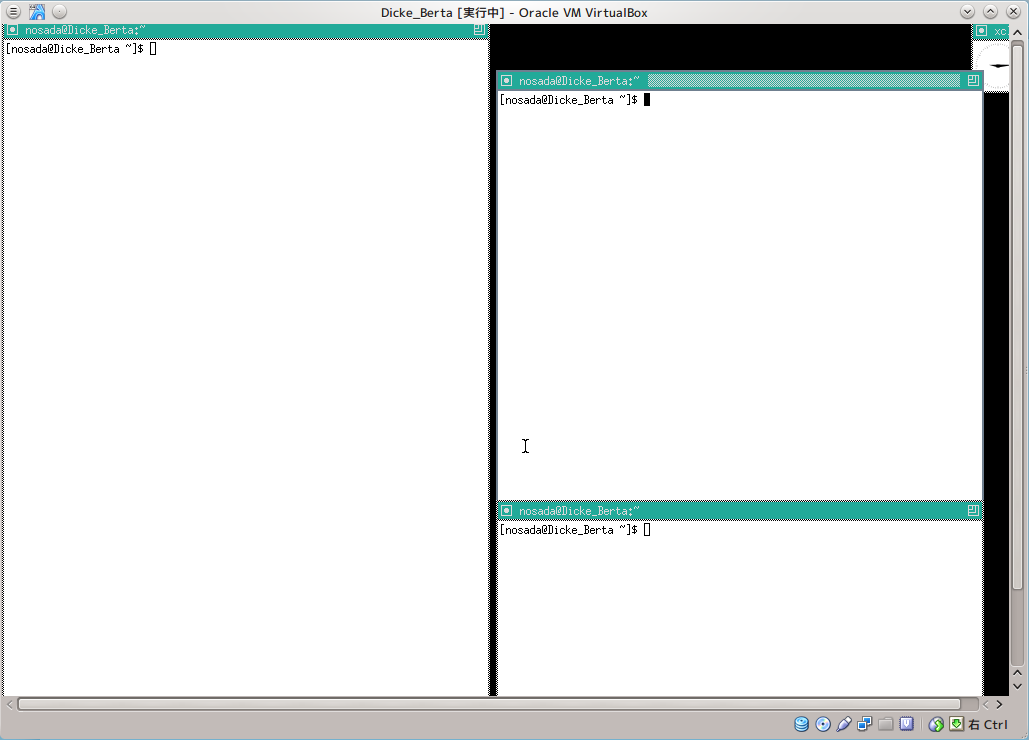
\includegraphics[scale=0.5]{Figs/Fig_ArchLinux/startx}\protect\caption{startx}
\label{startx}
\end{figure}



\subsection{GUIにおけるキーマップの再設定}

第\ref{chap:Arch-Linux=00306E=0030A4=0030F3=0030B9=0030C8=0030FC=0030EB}章でも触れた通り、CUIで設定したキー配列はGUIでは有効にならないことがあります。GUIにおいても適切なキー配列を設定する必要があるでしょう。ここではシステム再起動まで有効である一時的な設定と、永続的に有効である設定との2つを紹介します。


\subsubsection{一時的な設定}

とりあえず一時的でいいからキー配列を変えたいという場合、\texttt{setxkbmap}というコマンドを用いることができます。例えはキー配列をJIS配列にしたい場合、引数に``jp''を指定して、

\begin{center}
\shadowbox{\begin{minipage}[t]{0.6\textwidth}%
\texttt{\$ setxkbmap jp}%
\end{minipage}}
\par\end{center}

とすると良いでしょう。


\subsubsection{永続的な設定}

キー配列の変更を明示的に変更するには、Xの設定ファイルを編集する必要があります。Xの設定ファイルの場所は、概ね/etc/X11/xorg.conf.dです。ここを\texttt{ls}で確認すると、例えば10-evdev.confや10-quirks.confといった名前のファイルがあると思います。ここに置かれる設定ファイルは、名前が``\textless{}数値\textgreater{}-\textless{}名前\textgreater{}.conf''という命名規則に従うことを要求されます。このうち名前は適当でいいのですが、数値に関しては、既存のファイルに振られた数値よりさほど差がない値が良いでしょう。上の例であれば例えば20や30などが適当です。

さて、ここでは設定ファイルを``20-jpkbdmap.conf''として作成することにしましょう。名前は明快に``JaPanese
KeyBoarD MAPping''です。ここに、

\begin{center}
\doublebox{\begin{minipage}[t]{0.6\columnwidth}%
{\tt
\begin{tabbing}
12345\=6789012345678901 \kill
Section "InputClass" \\
	 \>Identifier "Keyboard Deults" \\
	 \>MatchIsKeyboard "yes" \\
	 \>Option "XkbLayout" "jp" \\
	 \>Option "XkbModel" "jp106" \\
EndSection
\end{tabbing}
}%
\end{minipage}}
\par\end{center}

と記述します。GUIを再起動すれば、設定は有効になるはずです。


\subsection{Xfceのインストール}

Xfce%
\footnote{\url{http://www.xfce.org/}%
}とは、前述したようにデスクトップ環境と呼ばれる、GUIを提供するソフトウェアです。XもGUIを提供するソフトウェアだと説明しましたが、例えるならXはコンクリート打ちっぱなしの内壁で、デスクトップ環境は断熱材や遮音材などを挟んで内装を整え、壁紙を貼った内壁のようなものです。すなわちXはGUIの基礎を構築し、Xの構築したGUIを用いて、デスクトップ環境はGUIを提供するのです。

Xfceをインストールするには、以下のように叩きます。

\begin{center}
\shadowbox{\begin{minipage}[t]{0.6\textwidth}%
\texttt{\$ sudo pacman -S xfce4 xfce4-goodies}%
\end{minipage}}
\par\end{center}


\subsection{LightDMのインストール}

LightDM%
\footnote{\url{http://www.freedesktop.org/wiki/Software/LightDM/}%
}とは、軽量なログインマネージャです。ログインマネージャとはシステムへログインするインターフェースのGUI版で、機能はCUIのログインインターフェースとそれほど変わるものではありません。ですが、ログインマネージャを導入した場合、マシンの電源を投入するとデスクトップ環境の起動に至るまでにコマンドを叩いたりする操作が不要になるので、使い勝手が少々よくなるという利点があります。

LightDMのインストールには、以下を叩きます。

\begin{center}
\shadowbox{\begin{minipage}[t]{0.6\textwidth}%
\texttt{\$ sudo pacman -S lightdm lightdm-gtk3-greeter xorg-server-xephyr}%
\end{minipage}}
\par\end{center}

インストール後、

\begin{center}
\shadowbox{\begin{minipage}[t]{0.6\textwidth}%
\texttt{\$ sudo systemctl enable lightdm.service}%
\end{minipage}}
\par\end{center}

と叩き、システム起動時にLightDMが起動するよう設定します。設定後、システムを再起動させれば、少々みすぼらしいですが、GUI上でログインが可能になっているはずです。


\subsection{Xfceの設定}

では早速Xfceを設定していきましょう。今回は本ゼミの目標である「ブラウザでgoogleを開いて日本語で検索ワードを入力して検索する」を達成する上で触れなければならない事柄について扱うにとどめます。他に必要があれば、本章末尾の補足で扱いたいと思います。

ちなみに、XfceでCUIによるコマンド操作を行うには、Xfce上でシェルを使用する必要が有ります。Alt+F2を入力してランチャを起動し、

\begin{center}
\shadowbox{\begin{minipage}[t]{0.6\textwidth}%
\texttt{xfce4-terminal}%
\end{minipage}}
\par\end{center}

とすることで、馴染み深いCUIが立ち上がります。ここでプログラムの起動に使用したのはシェルではなくランチャでありますので、上の操作においてプロンプトが表示されない事に注意して下さい。


\subsubsection{ロケールの再設定}

第\ref{chap:Arch-Linux=00306E=0030A4=0030F3=0030B9=0030C8=0030FC=0030EB}章で、CUIでのロケールは英語、GUIのロケールは日本語と個別に設定する、と述べましたが、どうもXfceではこのような設定は不可能なようです%
\footnote{筆者が普段使用しているKDEでは可能。理由がわからない。%
}。予想外の事態なのですが、思い悩んでも埒が明かないので、おとなしく/etc/locale.confを再設定しましょう。内容を``LANG=''ja\_JP.UTF-8''''に修正し、再起動します。ちなみに単純に

\begin{center}
\shadowbox{\begin{minipage}[t]{0.6\textwidth}%
\texttt{\$ nano /etc/locale.conf}%
\end{minipage}}
\par\end{center}

とすると、/etc/locale.confを編集できません。というのも、Linux上の全てのファイルにはファイルの管理者とパーミッションが定められており、基本的にシステムの設定ファイルはスーパーユーザが管理者となっています。加えて設定ファイルのパーミッションは、スーパーユーザに対してのみ書き込みが可能となっているので、一般ユーザが設定ファイルを編集する場合は\texttt{sudo}を用いなければなりません。

再起動後、システムは見事に日本語化されていると思います。


\subsubsection{UimとMozcの導入}

次に日本語を入力するためのIM%
\footnote{Input Method。文字通り多言語を「入力する手段」である。%
}であるUim%
\footnote{\url{https://code.google.com/p/uim/}%
}と、おそらく現在オープンソースのIME%
\footnote{Input Method Engine。言語を入力するためにIM中で駆動させるプログラム。%
}の中で最も性能の良いと思われるMozc%
\footnote{\url{https://code.google.com/p/mozc/}%
}をインストールします。

これには以下を叩きます。

\begin{center}
\shadowbox{\begin{minipage}[t]{0.6\textwidth}%
\texttt{\$ sudo pacman -S uim uim-mozc mozc}%
\end{minipage}}
\par\end{center}

インストール後、UimでMozcを使用するための設定を行います。まずCUI上で

\begin{center}
\shadowbox{\begin{minipage}[t]{0.6\textwidth}%
\texttt{\$ sudo uim-module-manager -{}-register mozc}%
\end{minipage}}
\par\end{center}

と叩き、UimにMozcを登録します。続いて

\begin{center}
\shadowbox{\begin{minipage}[t]{0.6\textwidth}%
\texttt{\$ uim-pref-gtk}%
\end{minipage}}
\par\end{center}

を叩き、UIMの設定ウィンドウを呼び出します。次に、「全体設定」中の「入力方式の利用準備」内にある「標準の入力方式を指定する」にチェックを入れ、「標準の入力方式」のプルダウンメニューからMozcを選択します。

続いて、Uimがシステム起動時%
\footnote{正確にはデスクトップ環境の起動時。%
}に自動的に立ち上がるように設定します。/home/\textit{USERNAME}/.xprofile(\textasciitilde{}/.xprofileと同義)の末尾に以下を追記します。

\begin{center}
\doublebox{\begin{minipage}[t]{0.6\textwidth}%
\texttt{export GTK\_IM\_MODULE='uim' }

\texttt{export QT\_IM\_MODULE='uim' }

\texttt{uim-xim \& }

\texttt{export XMODIFIERS='@im=uim'}

\texttt{uim-toolbar-gtk-systray \&}%
\end{minipage}}
\par\end{center}

ただし、初期状態では恐らく当該ファイルはディレクトリ上に存在しないので、

\begin{center}
\shadowbox{\begin{minipage}[t]{0.6\textwidth}%
\texttt{\$ nano \textasciitilde{}/.xprofile}%
\end{minipage}}
\par\end{center}

として、.xprofileを作成する必要があります。この方法でファイルを作成すると実際にファイルへの変更を保存するまでファイル自体は作成されないことに注意して下さい。なお、.xprofileのようにファイルの先頭に``.''(ドット)がつくファイルは隠しファイルと呼ばれるもので、通常の手段(単に\texttt{ls}と叩くなど)では表示されません。隠しファイルを表示させる場合、\texttt{ls}では\texttt{-a}オプションを付けます。GUI上のファイラではファイラの操作方法に依存するので一概に言えません。

追記後、システムを再起動させれば、日本語入力が可能となっているはずです。日本語入力の入切は全角/半角キーで、Uim自体の入切はAlt+Spaceで可能です。キーバインドは任意で変更可能ですから、設定を使いやすいように変更するのも良いでしょう。


\subsubsection{ブラウザの導入}

最後にブラウザの導入です。ブラウザにはMidori%
\footnote{\url{http://www.midori-browser.org/}%
}を使用します。Midoriは

\begin{center}
\shadowbox{\begin{minipage}[t]{0.6\textwidth}%
\texttt{\$ sudo pacman -S midori}%
\end{minipage}}
\par\end{center}

とすることでインストールができます。

ブラウザの起動方法は、デスクトップ右上の「アプリケーションメニュー」から「インターネット」を選択し起動するのも良いですが、\texttt{xfce4-terminal}を起動したようにAlf+F2を入力した後

\begin{center}
\shadowbox{\begin{minipage}[t]{0.6\textwidth}%
\texttt{midori}%
\end{minipage}}
\par\end{center}

と叩いても起動することができます。

では、いよいよ本ゼミの最終目標である、「ブラウザでgoogleを開いて日本語で検索ワードを入力して検索する」を実践したいと思います。とはいっても普段皆さんが普段使用しているブラウザで行っているのと同様に、ブラウザのアドレスバーに\url{http://www.google.com}と入力し、表示されるgoogleの検索ボックスに適当な検索ワードを入力し、Enterを押下するだけです。これで、Arch
Linux上に構築したGUIにおいてブラウザを起動し、ブラウザでgoogleにアクセスし、googleの検索ボックスに日本語で検索ワードを入力し、検索を行う、という本ゼミの目標を達成することが出来ました。

\begin{figure}[!tbh]
\centering{}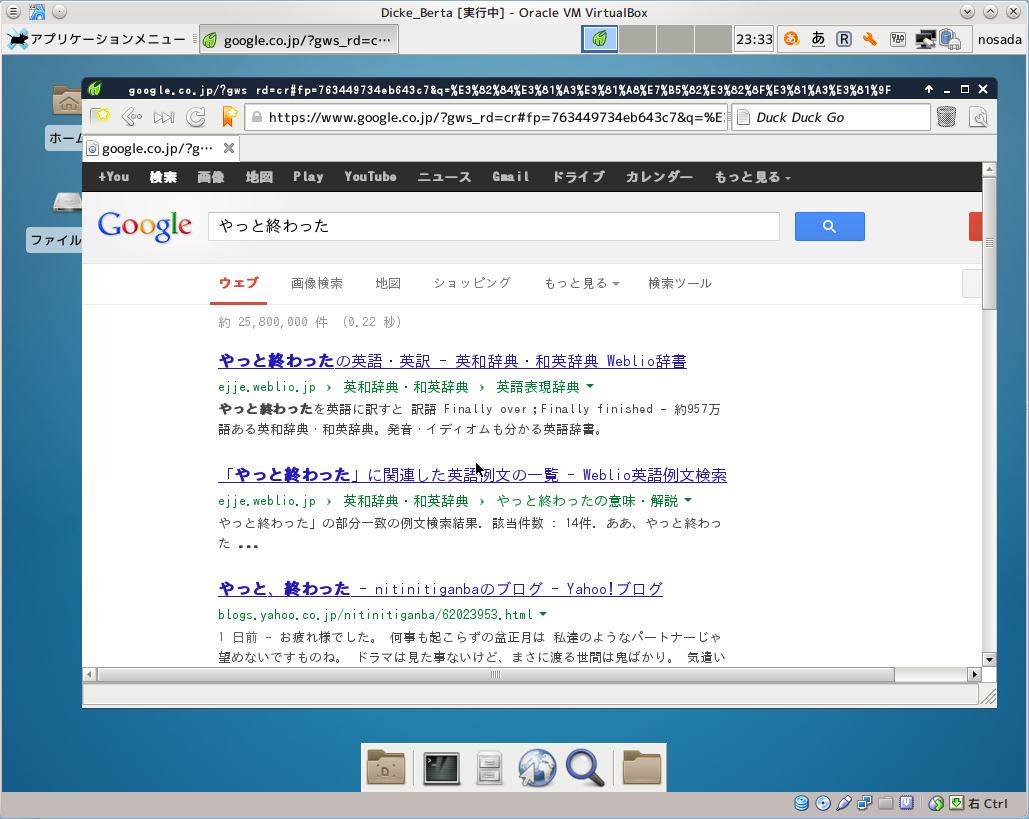
\includegraphics[scale=0.5]{Figs/Fig_ArchLinux/finished}\protect\caption{やっと終わった。}
\label{Finally_Finished}
\end{figure}



\section{補足}

ここではArch Linuxを常用する上で知っておくべきであろう事柄について、簡単に触れていきたいと思います。

この節では説明を簡略化する代わりに、各項目に対応したArchWikiのURLを添えておきます。興味をお持ちになった際は、ArchWikiの当該項目で詳細をご覧ください。


\subsection{AURの利用\protect \\
(\protect\url{https://wiki.archlinux.org/index.php/AUR})}

Arch Linuxには、Arch Linux本家が管理運用するレポジトリの他に、Arch Linuxのユーザがパッケージを作成するためのファイル(PKGBUILD)を投稿するAUR(Arch
User Repository)%
\footnote{\url{https://aur.archlinux.org/}%
}というものがあります。ここには主にライセンスの都合上本家のレポジトリには登録できないパッケージや、本家に登録されているパッケージの不安定版、あるいは既存のパッケージに機能を追加するためのパッケージであったり、ジョークプログラムを収めたパッケージであったりと、多種多様なパッケージが登録されています。この多種多様というワードが示す通り、使用したいと思ったパッケージが公式レポジトリになくても、AURを探せば大抵見つかるという便利さも兼ね揃えています。

このAURですが、残念ながら\texttt{pacman}から直接では利用することができません。利用する場合、AURにアクセスし、インストールしたいパッケージを探し、そのパッケージを作成するためのPKGBUILDが含まれた圧縮ファイルを入手し、解凍、パッケージ作成、インストールという手順を踏まなければなりません。

ですが、\texttt{pacaur}%
\footnote{\url{https://wiki.archlinux.org/index.php/Pacaur}%
}という\texttt{pacman}のラッパプログラムを用いれば、\texttt{pacman}と同じような使い方でAURにアクセス、PKGBUILDをダウンロードすることができます。

ところで、おそらく図\ref{Finally_Finished}はあなたが構築したデスクトップ環境に比べ、フォントが綺麗なものになっていると思います。AURにはこのようなフォントデータも大量に転がっており、わざわざインターネット上からフォントを探し出してインストールしなくても、シェル上でコマンドを叩くだけで導入が可能なのです。


\subsection{ネットワーク接続の管理\protect \\
(\protect\url{https://wiki.archlinux.org/index.php/Network_Configuration})}

実機へのArch Linuxを行った場合、特にノートパソコンなどではインターネットへの接続に無線接続を用いることが多いと思います。そのような場合などの汎用性を鑑みて、補足としてwicd%
\footnote{\url{http://wicd.sourceforge.net/}%
}というネットワーク接続管理ソフトウェアのインストールを扱います。この操作は必ずしも必須ではありません。

まず以下のように叩き、wicdとwicdの動作に必要なパッケージをインストールします

\begin{center}
\shadowbox{\begin{minipage}[t]{0.6\textwidth}%
\texttt{\$ pacman -S wicd}%
\end{minipage}}
\par\end{center}

インストールが終了したら、次に以下のように叩き、wicdデーモンを有効化します。

\begin{center}
\shadowbox{\begin{minipage}[t]{0.6\textwidth}%
\texttt{\# systemctl enable wicd.service}%
\end{minipage}}
\par\end{center}

最後に、wicd以外のネットワークデーモンを停止、無効化します。これはwicd以外のネットワークデーモンが動作している場合、wicdの動作に支障を来すおそれがあるためです。この操作と上の操作は、環境によって前後する場合があります。適宜調整してください。具体的にはこの文書の順序に従ってエラーが発生した場合、順番を入れ替えて実行してください。

\begin{center}
\shadowbox{\begin{minipage}[t]{0.6\textwidth}%
\texttt{\# systemctl stop dhcpcd.service}

\texttt{\# systemctl stop netctl.service}

\texttt{\# systemctl disable dhcpcd.service}

\texttt{\# systemctl disable netctl.service}%
\end{minipage}}
\par\end{center}

\begin{center}
これで使用準備は完了です。実際に使用可能になるのはインストール完了後に再起動した後になります。
\par\end{center}

wicdをCUIで使用する場合は

\begin{center}
\shadowbox{\begin{minipage}[t]{0.6\textwidth}%
\texttt{\$ wicd-curses}%
\end{minipage}}
\par\end{center}

と叩くとインターフェースが起動します。GUIで使用する場合は、例えば今回のようにXfceなどのGTK系のツールキットを使用しているデスクトップ環境の場合は、

\begin{center}
\shadowbox{\begin{minipage}[t]{0.6\textwidth}%
\texttt{\$ sudo pacman -S wicd-gtk}%
\end{minipage}}
\par\end{center}

と叩き、\texttt{wicd-gtk}を使用すると良いでしょう。

無線接続などの詳細な設定は扱いません。\url{https://wiki.archlinux.org/index.php/Wireless_Setup}を参照するのが手っ取り早いでしょう。wicdについては\url{https://wiki.archlinux.org/index.php/Wicd}が役立ちます。


\subsection{音を鳴らす\protect \\
(\protect\url{https://wiki.archlinux.org/index.php/Sound})}

Arch Linux上でサウンドシステムを扱うには、ALSA%
\footnote{\url{http://www.alsa-project.org/main/index.php/Main_Page}%
}とOSS%
\footnote{\url{http://www.opensound.com/}%
}の2種類の手段があります。通常はLinuxカーネルの構成部品の一つであるALSAを使用するのが良いでしょう。ここではALSAについて触れます。

ALSAを使用するには、

\begin{center}
\shadowbox{\begin{minipage}[t]{0.6\textwidth}%
\texttt{\$ sudo pacman -S alsa-utils}%
\end{minipage}}
\par\end{center}

と叩いてALSAを触るためのユーティリティをインストールし、

\begin{center}
\shadowbox{\begin{minipage}[t]{0.6\textwidth}%
\texttt{\$ alsamixer}%
\end{minipage}}
\par\end{center}

を叩きます。CUIで表示されるミキサー画面を適当に弄くり回せば十分でしょう。デフォルトでは全てのパラメータがミュートされていますが、Mキーによりミュートをオン・オフできます。

ALSAについては\url{https://wiki.archlinux.org/index.php/Advanced_Linux_Sound_Architecture}を、OSSに関しては\url{https://wiki.archlinux.org/index.php/Open_Sound_System}を参照すると良いでしょう。
\begin{thebibliography}{10}
\bibitem[1]{LSP}Robert Love 著, 千住治郎 訳, 『LINUXシステムプログラミング』(オライリー・ジャパン,
2011)

\bibitem[2]{OS}Abraham Silberschatz, Peter Baer Galvin, Greg Gagne,``Operating
System Concepts 9th Edition''(John Wiley \& Sons, Inc., 2013)

\bibitem[3]{LST}岡田健治, 川井義治, 宮原徹, 佐久間伸夫, 遠山洋平, 田口貴久, 松田神一, 木村真之介,
高橋征義, 『Linux標準教科書(ver2.0.0)』(LPI--Japan, 2012)\\
\url{http://www.lpi.or.jp/linuxtext/text.shtml}

\bibitem[4]{ALBG}『Beginners' Guide - ArchWiki』\\
\url{https://wiki.archlinux.org/index.php/Beginners'_Guide}

\bibitem[5]{ALIG}『Installation Guide - ArchWiki』\\
\url{https://wiki.archlinux.org/index.php/Installation_Guide}

\bibitem[6]{AL}『Arch Linux - ArchWiki』\\
\url{https://wiki.archlinux.org/index.php/Arch_Linux}

\bibitem[7]{LINUX}『Linux - Wikipedia』\\
\url{http://ja.wikipedia.org/wiki/Linux}

\bibitem[8]{UNIX}『UNIX - Wikipedia』\\
\url{http://ja.wikipedia.org/wiki/UNIX}

\bibitem[9]{HOL}『History of Linux - Wikipedia, the free encyclopedia』\\
\url{http://en.wikipedia.org/wiki/History_of_Linux}

\bibitem[10]{ALK}『About Linux Kernel』\\
\url{https://www.kernel.org/linux.html}

\bibitem[11]{GNU}『GNU - Wikipedia』\\
\url{http://ja.wikipedia.org/wiki/GNU}

\bibitem[12]{GOS}『GNUオペレーティング・システムについて - GNUプロジェクト - フリーソフトウェアファウンデーション』\\
\url{http://www.gnu.org/gnu/about-gnu.html}

\bibitem[13]{DoFS}『自由ソフトウェアとは? - GNUプロジェクト - フリーソフトウェアファウンデーション』\\
\url{http://www.gnu.org/philosophy/free-sw.html}

\bibitem[14]{BSD}『BSD - Wikipedia』\\
\url{http://ja.wikipedia.org/wiki/BSD}

\bibitem[15]{MINIX}『Minix - Wikipedia』\\
\url{http://ja.wikipedia.org/wiki/Minix}

\bibitem[16]{LD}『Linux distribution - Wikipedia, the free encyclopedia』\\
\url{https://en.wikipedia.org/wiki/Linux_distribution}

\bibitem[17]{FHS}『Filesystem Hierarchy Standard』\\
\url{http://www.pathname.com/fhs/pub/fhs-2.3.html}

\bibitem[18]{AFH}『Arch filesystem hierarchy - ArchWiki』\\
\url{https://wiki.archlinux.org/index.php/Arch_filesystem_hierarchy}

\bibitem[18]{AP}『Partitioning - ArchWiki』\\
\url{https://wiki.archlinux.org/index.php/partitioning}

\bibitem[19]{An}『netctl - ArchWiki』\\
\url{https://wiki.archlinux.org/index.php/netctl}\end{thebibliography}

\end{document}
